
%% REMBER C4 TEMP! RADS.

%% TODO: in time, Make plot of proportion of extinctions by FG.
%% TODO: intro to initial results: do we refer forwards to dependence on IR?
%% TODO: comment on random but not systematic error - related to Alan's comment in email.
%TODO: nonte on veg predators - fixed  here
%TODO: link up these section references. (and add recent papers into .bib file) \\
%TODO: finish discussion of results. But first redo analysis with averaging? 
%TODO: look at "effective immigration" rates..? (inversley proportional to total biomass)
%TODO: show some results here for 0 HL
%TODO: look at longer runs (steady-state)
%TODO: look at over-abundance of top trophic level (re-run results)
%TODO: averaging of RADS (and others..) WAIT FOR STEADY STATE.
%TODO: either end each section with ecological context and implications, or have in separate section after results.
%TODO: finds out about Kevin McCann on omnivory (biomass pyramids?)
%
%\section{New predictions (Temp)}
%
%New predictions and questions following on from previous chapters, which are now basically complete. Need to make this chapter follow on nicely, and demonstrate improved understanding of the model!
%
%\begin{itemize}
%	\item At lower IR we should start to see more extinctions along the HL gradient
%	
%	\item Contiguous HL did not change community structure (RA,diversity,evenness,network metrics). Only interaction strengths and variability changed (not synchrony). However we expect that, along the IR gradient these properties will change, due to less input from immigration which as we saw is a levelling influence. Therefore we expect communities to become less even, and perhaps more aggregated in space (although we cannot test the latter..we could maybe..)
%	
%	\item Following from above: can we find an IR where we see interesting behaviour along the HL gradient, either extinctions or changes in community structure (not just changes in variability). Is there a critical threshold for IR beyond which this occurs? 
%	
%	\item We know from previous chapter that dynamics becomes more variable, but also more deterministic, with reduced IR. Is this associated with increased interaction strengths? How does this carry across along the HL gradient? What does synchrony tell us (or determinism tests?)
%	 
%\end{itemize} 

%\section{Assumptions of what has gone before}
%
%% Daniel's main feedback is 1) be more assertive and positive about the work, 2) be more explicit about it relationship the nature.
%
%\begin{itemize}
%
%	\item Conclusion that the ddefault immigration rate is high and this is an open system. This represents a restricted scenario where the regional species pool is constant and high (60 species), all species are equally likely to immigrate and dispersal from outside our 'world' is not heavily constrained. In this chapter we look at varying immigration rates, habitat loss and MAI.
%	\item A discussion of the "rescue effect" due to immigration. Probability of species spawning. Effective immigration, although currently that concept is first mentioned in this chapter.
%	\item Context of `viable species' as opposed to those that only remain due to immigration `bubbling' along close to zero. (note that this is quite realistic)
%	\item Snapshots of system versus averaging of metrics over a number of iterations (seems a bit late in the thesis to realise that this is a problem in chapter 4!) - averaging over replicates can justify this to some extent (25 in previous chapters, 100 here).
%	\item It may be that this model is well approximated by GLV. If so it would make sense to discuss the results with reference to that? Should try to fit?
	
%\cite{ripple2012trophic}

%% RESUCE EFFECT:
%%THIS FOR LATER: (WHERE?) It is important to note that even at low IR species which go extinct during the simulation may be rescued. Therefore it is interesting to ask how much of this persistence in higher trophic levels is due immigration rescue effects. These could lead to a situation with a number of very rare species 'bubbling along' close to zero (becoming extinct and then being rescued), with a small core of more abundant species meaningfully engaged in interaction dynamics and demographic processes\footnote{If this is the case it leads intuitively to the concept of 'viable' species, possibly more useful here than 'non-extinct'.}.

\section{Motivation}
\label{sec:motivate_immigration}

In chapter \ref{chap:habitat_loss_high_immigration} we discovered that the immigration mechanism provides a \emph{rescue effect} for all species, preventing extinctions even at high levels of habitat loss (HL$=90\%$). This allowed us to study community responses to HL in the absence of extinctions. However in nature it is common that HL does lead to the local loss of species \cite{foley2005global}. Therefore we are motivated to reduce the immigration rate (IR), weakening the rescue effect, to study communities in which HL results in extinctions. In chapter \ref{chap:stress_testing} we found that communities at zero IR - \emph{closed communities} - displayed many extinctions, even in pristine landscape. We concluded that some immigration is required for the IBM to produce persistent and diverse communities. Therefore in this chapter we study the response of communities to HL at IRs between zero and the \emph{default value} ($IR=0.005$). We expect that varying the immigration rate will cause community responses to HL to differ from those observed in chapter \ref{chap:habitat_loss_high_immigration}. In particular we are interested to study community responses to HL when species extinctions are allowed to occur.

In the previous analysis we have demonstrated that immigration is a key determinant of the dynamics and structure of simulated communities. In chapter \ref{chap:stress_testing} we saw that high IR reduces both the temporal variability and the determinism of population dynamics. In chapter \ref{chap:habitat_loss_high_immigration} we demonstrated that strong immigration acts to increase the evenness in the distribution of species abundances and that this can affect network properties, for example by making interaction frequencies more even. In particular we saw that the \emph{dependence of a community on immigration} (measured by the relative contribution of immigration to total births) could account for the different structural responses of communities under the two HL scenarios. The contiguous HL scenario did not produce significant changes in many of the metrics analysed, and it was argued that this was due to the constant dependence of communities on immigration across the HL gradient. In contrast random HL increased community dependence on immigration, and produced significant changes in most of the metrics analysed. In this chapter we employ the same two HL algorithms (section \ref{sec:model_HL}), \emph{random} and \emph{contiguous}, at a range of different IRs. We anticipate that reduced IR may effectively reduce community dependence on immigration in some cases. In such cases we hypothesise that HL will make communities less even, and that there will be corresponding changes in network properties. It is most likely that such an effect will be found in the contiguous scenario, because intra- and inter-specific interactions remain strong under contiguous HL. This observation was discussed in detail in section \ref{sec:res_synthesis}, but the main arguments are summarised below.

Species interactions have proven to be another key driver of population dynamics and community structure, as expected. In chapter \ref{chap:habitat_loss_high_immigration} strong inter-specific interactions, as measured by IS, were shown to produce high temporal variability. In chapter \ref{chap:stress_testing} it was demonstrated that this variability was due to deterministic oscillations, characteristic of predator-prey interactions. We have also found that the two HL scenarios have different effects on species interactions due to changes in the mobility of individuals (figure \ref{fig:diffusion_example}). Random HL presents a barrier to motion making both inter- and intra-specific interactions less likely. This accounts for the increased dependence on immigration in the random scenario, since sexual and mutualistic reproduction is hindered by the destroyed cells, which act as physical barriers and make it difficult for individuals to find a mate. Contiguous HL makes interactions more likely because all individuals are contained within a smaller region of space and maintain the same dispersal ability. Therefore in the contiguous scenario at low IR we may expect to see a reduced dependence on immigration, and increase in the effects associated with strong species interactions. Conversely we may expect low IR to weaken the effects of random HL, which were associated with increased dependence on immigration at the default IR value.   

In general we anticipate that reducing IR will strengthen the effects associated with species interactions, and weaken those associated with immigration. In particular we expect communities to become less even and more temporally variable as IR is reduced. There may also be an increase in \emph{ecosystem synchrony} as the stochastic component of the dynamics is reduced relative to the deterministic component. Such effects should be visible at any given HL value under both scenarios. Finally we expect that at lower IRs both HL scenarios will generate species extinctions. 

In section \ref{sec:exp_method} we detail the experimental methodology for the chapter, including an experiment to determine how to sample from the simulation output (section \ref{sec:estimators}) given the increased variability expected from reduced IR (see chapter \ref{chap:stress_testing}). Section \ref{sec:init_res} presents an initial analysis of certain key metrics over a slice of the IBM parameter space defined by varying IR and HL. Sections \ref{sec:biv_fixIR} and \ref{sec:biv_fixHL} develop the initial analysis further by conducting bivariate analyses at selected IR and HL values respectively.  We summarise the main findings of the chapter in section \ref{sec:vir_discussion}, before concluding in section \ref{sec:vir_conclusion} with an ecological interpretation of the perspectives gained from our simulations of the IBM.

%It may be possible to detect the stabilising role of immigration explicitly. That is, at a given HL value, IS may be constant as IR is reduced, but the dynamics becomes more variable.

%
%\begin{figure}
%	\centering
%	\includegraphics[width=0.8\linewidth]{"figures/hist_species_per_tl_zeroIR"}
%	\caption{Fractional persistence by trophic level for three different MAI ratios. Fractional persistence is measured by the fraction of speices intially belonging to a trophic level which have not gone extinct by the end of a simulation (5000 iterations). The solid bars give the mean value, taken  from 22 repeat simulations. Error bars show $\pm$ one standard deviation. (Simulations from chapter \ref{chap:stability}}
%	\label{fig:mvp_hist_zeroIR}
%\end{figure}


\section{Experimental approach}
\label{sec:exp_method}

As in chapter \ref{chap:habitat_loss_high_immigration} we run two ensembles of simulations, one for random and one for contiguous HL. The value of HL  is varied between $0\%$ and $90\%$ in steps of $10\%$, as before. At each value of HL we run replicates at 10 different immigration rates: IR$ = 1 \times 10^{-4},2 \times 10^{-4},3 \times 10^{-4},4 \times 10^{-4},5 \times 10^{-4},1 \times 10^{-3},2 \times 10^{-3},3 \times 10^{-3},4 \times 10^{-3},5 \times 10^{-3}$. Therefore each ensemble explores a two-dimensional slice of the parameter space, defined by the axes HL and IR. This same region of parameter space was visualised in figure \ref{fig:nssp_ir_v_hl} during the stationarity testing. The inclusion of variable IR increases the number of required simulations by a factor of ten, compared to the simulation ensemble of chapter \ref{chap:habitat_loss_high_immigration}. To reduce the computational cost we make two savings. Simulations are only run for three MAI ratios ($0.0,0.5,1.0$) instead of eleven, giving the full range between antagonism and mutualism but with lower resolution. Additionally we restrict the number of metrics that are calculated during each simulation. The spatial metrics in particular are computationally expensive. Therefore all of the metrics defined in section \ref{sec:def_spatial_metrics}, which characterise spatial aggregation and variability, are not calculated. This speeds up the simulation run times by about a factor of five, but means that we cannot characterise spatial patterns without \emph{post-hoc} analysis.

In section \ref{sec:reliability} it was shown that the increased temporal variability resulting from reduced IR can make results more sensitive to the sampling procedure. It may be desirable to run the simulations for an increased number of time steps, allowing for longer samples from which to calculate results. However it was decided that this is an unnecessary computational expense. The regression analysis of estimator quality suggested that a sample length of 4000 characterises species abundances with reasonable accuracy ($E(R^2) > 0.9$) in pristine landscape at low IR ($1 \times 10^{-4}$). Therefore all simulations in this chapter were run for 5000 time steps, with the first 1000 time steps discarded before analysis (as in chapters \ref{chap:habitat_loss_high_immigration}, \ref{chap:stress_testing}). In section \ref{sec:init_res}, before presenting the main results, we further address the issue of sampling procedure by statistically comparing results obtained using two different sampling methods. 

In this chapter the number of replicate simulations is increased from 25 (used in chapter \ref{chap:habitat_loss_high_immigration}) to 50. The use of a higher number of replicates reflects the previous observation of increased variability, and therefore a larger source of random error in the results. With 50 replicates at every value of HL, IR and MAI ratio, each ensemble contains $15,000$ ($= 50 \times 10 \times 10 \times 3$) simulations. Each replicate uses a distinct interaction network generated using the same procedure as in chapter \ref{chap:habitat_loss_high_immigration}, that is a niche model with trophic constraints and link replacement to introduce mutualisms (details in section \ref{sec:interaction_network}). The only modification is that here links between top-predators and basal species are removed from the network, so that top-predators only feed on other animal species. On average such links represented less than five percent of the total links in a network (calculated from the ensemble of simulations used in chapter \ref{chap:habitat_loss_high_immigration}). Therefore we not expect a qualitative change in the main findings presented in chapters \ref{chap:habitat_loss_high_immigration} and \ref{chap:stress_testing}. As previously all simulations were run on the Blue Crystal cluster \cite{BC3}.

Given that we are interested in species extinctions induced by HL, in this chapter we redefine the definition of a local \emph{extinction}. Previously a species was said to be extinct if there were no individuals belonging to that species in the landscape at the end of the simulation. However we have seen that immigration provides a \emph{rescue effect} that is common to all species. A species may go extinct at some time in the simulation, but later recover due to immigration. For example a species may be extinct for most of the simulation and then an immigrant belonging to this species is created on the final time step. The previous definition of extinction would not count such a species as extinct. Especially at low IR we expect many species to have abundances that hover close to zero. We make the assertion that such species are effectively locally extinct because they fail to maintain a viable local population and are only sustained by immigration. Indeed, in an empirical study sufficiently rare species are unlikely to be detected and therefore do not contribute to estimates of species richness. Therefore it is felt that the previous definition of species extinction does not correctly characterise the state of the system. We propose a new definition of extinction as follows. A species  is declared extinct if its population size (or average population size if sampling over a number of time steps) is lower than a specified \emph{threshold value}. In section \ref{sec:init_res} we set an \emph{arbitrary threshold} of three individuals. Subsequently in section \ref{sec:extinction} we revisit this definition of extinction and the choice of the threshold value.

%Therefore our previous definition of extinction, as the absence of any individuals belonging to a given species, proves problematic. Snapshot measurements of species on the border of extinction will be particularly sensitive to the time at which the measurement is taken. Measurements of abundance made by averaging over a number of time steps will result in small but non-zero population sizes for borderline species. Requiring that a species population size is at zero will therefore mean we again detect no extinctions. In the initial analysis (section

%NOTE: on vegetarian predators! $<5\%$ of links on average, so should not make too much difference\footnote{Need to recalculate proportions.}.
%ALSO: will be used RADs, or just Shannon? Why?

%From previous chapter we know that need long term averages. Problem: network metrics still only calculated over 200 iterations. Do a comparison of some results 200 vs 4000 iterations?

\subsection{Sampling procedure}
\label{sec:estimators}
%% This figure produce by:(uni)/MyFiles/cm1788/Documents/IM_vs_HL_heatmap/clean_results/random/plot_pval.py
\begin{figure}
	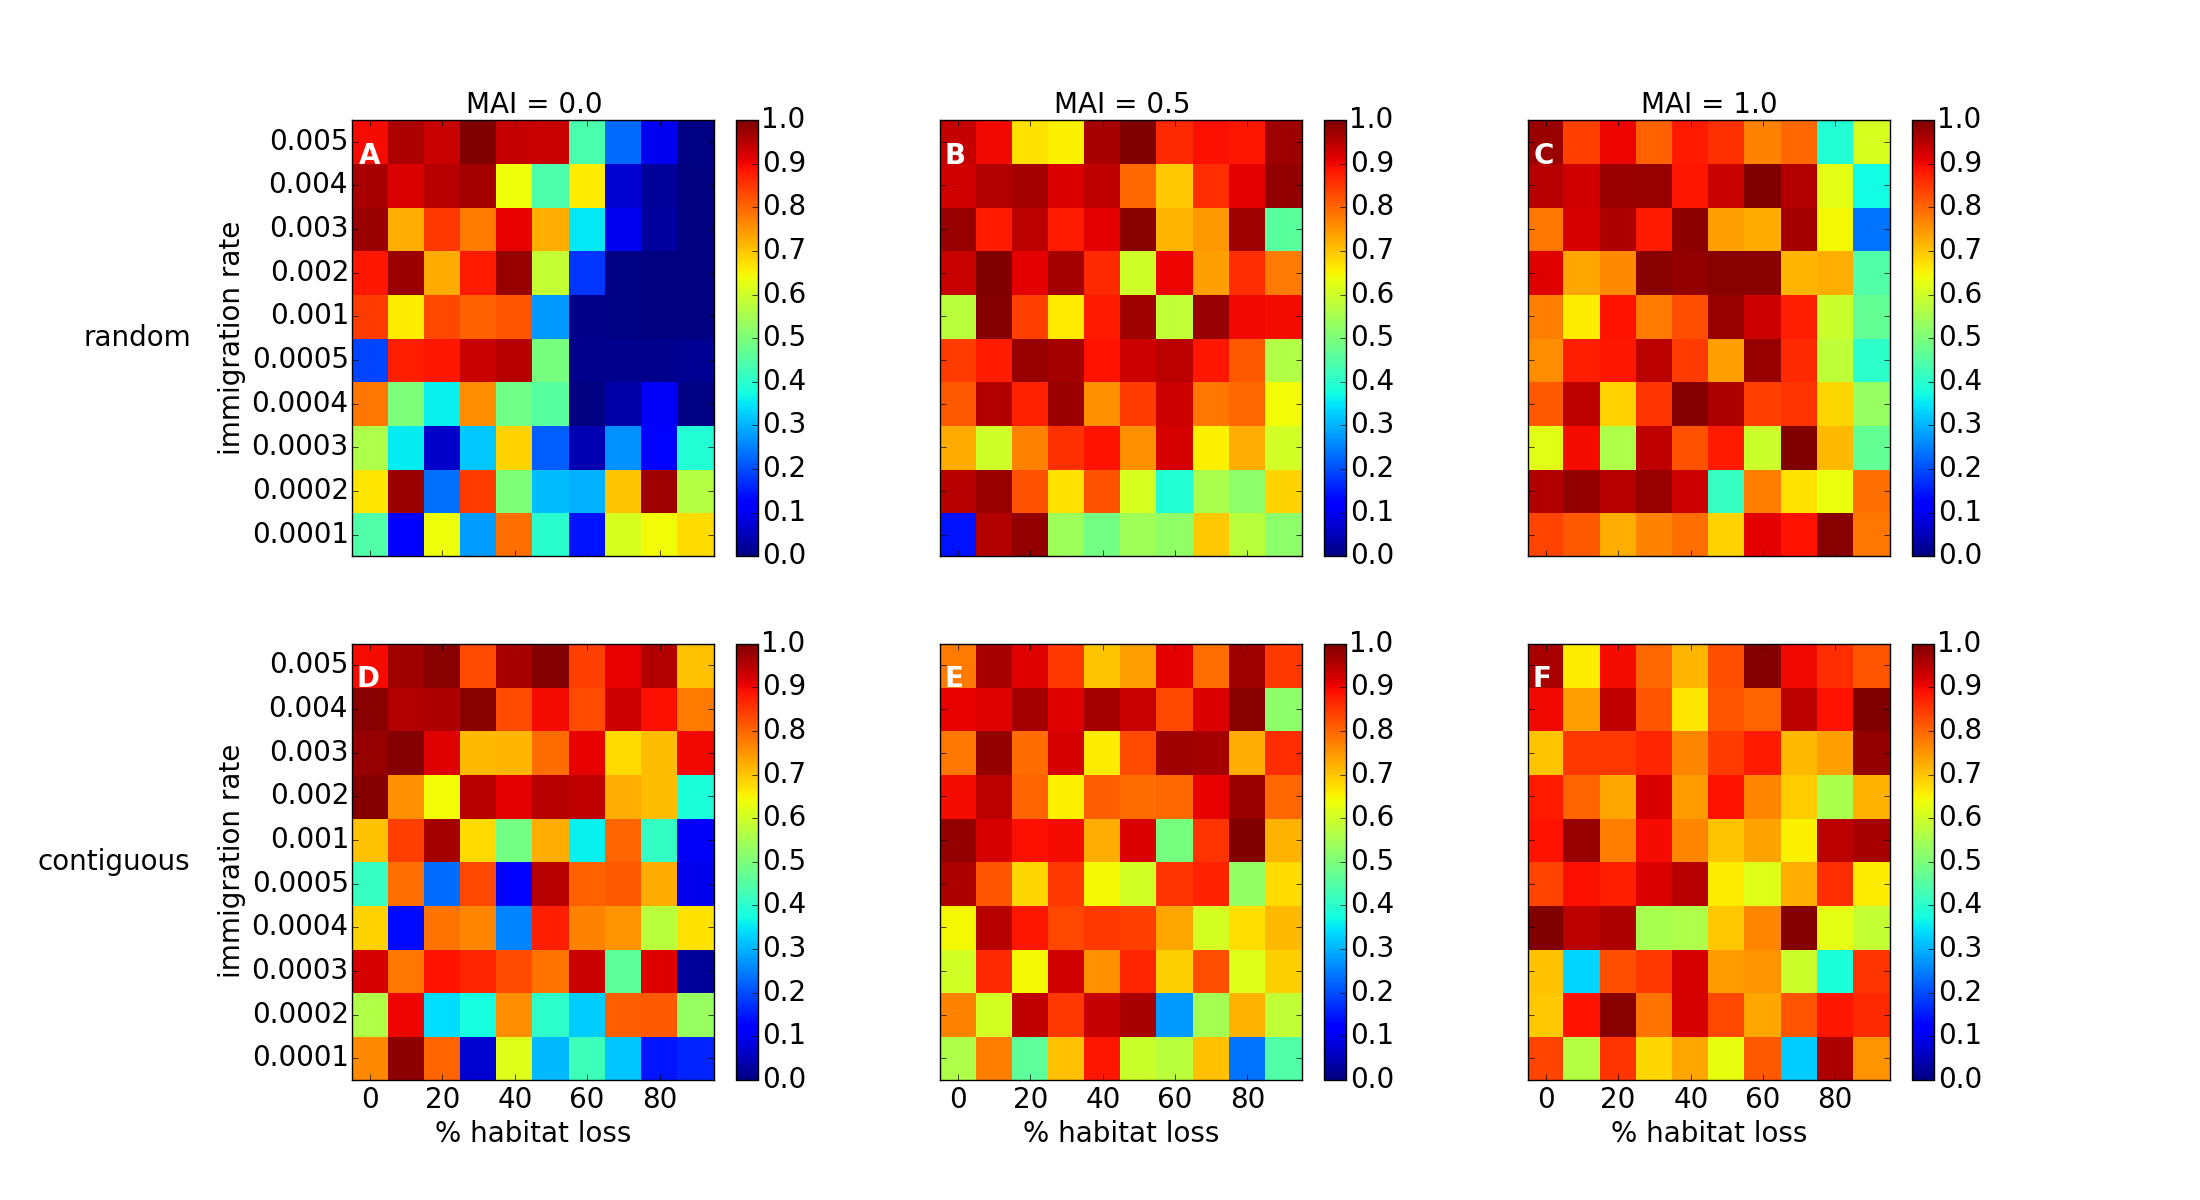
\includegraphics[width=\textwidth]{{{figures/clean_analysis/heatmap_ttest}}}
	\caption{P-values for t-tests to compare the \emph{Shannon equitability} calculated by two different sampling methods: \emph{snapshot} and \emph{averaged} sampling (see text for definitions). Each point in the plot represents the p-value of the test comparing the \emph{snapshot} and \emph{averaged} Shannon equitability results for the 50 replicate simulations at the corresponding HL and IR value. A p-value$<0.05$ (i.e.dark blue) represents $95\%$ confidence that the two sampling methods produce different average equitability results.}
	\label{fig:ttest}
\end{figure}

The \emph{Shannon equitability} metric (equation \eqref{eq:shan_eq}) is calculated for all simulations using two different sampling methods. The first method uses snapshot sampling (as in chapter \ref{chap:}), i.e. species abundances are measured on the last time step of the simulation. The second method takes the mean species abundance over the final 4000 time steps of the simulation. Results obtained using the two sampling methods are referred to as \emph{snapshot} and \emph{averaged}, correspondingly. We compare the results obtained using a \emph{two-sided t-test}, which is implemented in the \emph{Python} package \emph{scipy}. The test is used to compare two datasets of independent samples, testing the null hypothesis that the expected value of the two datasets are equal. If the \emph{p-value} of the test is smaller than the confidence threshold then there is sufficient evidence to reject the null hypothesis and conclude that the means of the two datasets are significantly different. For each test we are comparing the \emph{snapshot} and \emph{averaged} equitability results, calculated from the 50 replicate simulations at a given HL and IR value. If the test is significant then we conclude that the two sampling methods give significantly different results in calculation of the average Shannon equitability at that value of HL and IR. We conduct tests for all HL and IR values, and all three MAI ratios, under random and contiguous HL. The \emph{p-values} of these tests are depicted in figure \ref{fig:ttest}.  

In general figure \ref{fig:ttest} shows that there is strong support for the conclusion that the two sampling methods produce the same average equitability results. The worst case is random HL at MAI$=0.0$ (panel A). In this case there is a region of parameter space, above HL$=60\%$, where the p-values are significant. Therefore in this region the methods appear to give statistically different results. However, as stated, most of the tests suggest that the two methods produce statistically similar results. The similarity between the two methods is surprising given the results of the estimator analysis in section \ref{sec:convergence}. In part the success of the snapshot method is likely due to averaging over 50 replicates, which effectively represent samples from the same noise distribution. It may also be that a high level of precision in the estimates of species abundances is not required to calculate community level metrics. Based on the comparison presented here we conclude that snapshot sampling is sufficient to draw general conclusions about community structure over the ensemble of simulations. This allows consistency with the analysis in chapter \ref{chap:habitat_loss_high_immigration}. However we acknowledge that the use of snapshot samples may introduce some error, and increased variability, into our calculations. We treat the region of parameter space in which the equitability results proved dissimilar (panel A: random HL. MAI$=0.0$) with particular caution\footnote{remember to caution the stated area!}. The metrics for network properties (defined in section \ref{sec:define_network_metrics}) and stability (defined in section \ref{sec:def_stability_metrics}) are calculated by aggregating over the final 200 time steps of a simulation, as in previous chapters. We do not provide an equivalent statistical comparison of these metrics when calculated from samples of different lengths. Given that these metrics already use a sample of length 200, we assume that they are less sensitive than the snapshot metrics to error introduced by high variability.   

\section{Initial analysis}
\label{sec:init_res}

In this section we provide an overview of the results for both the random and contiguous scenarios, over the region of parameter space explored. Results are presented as \emph{heat-maps} over parameter space. Each pixel corresponds to a unique pair of HL and IR values, with the temperature (colour) given by the corresponding mean value of the metric in question (averaged over the 50 replicates). In this way it is possible to gain a qualitative impression of how the various metrics respond as HL and IR are varied. In sections \ref{sec:vir_diversity} and \ref{sec:vir_variability} we provide results for selected metrics associated with diversity, and variability respectively. In subsequent sections we look in more detail at key features identified from the initial analysis presented here. All results presented use the same sampling procedure as in chapter \ref{chap:habitat_loss_high_immigration}, i.e. snapshot samples for abundance metrics and sample lengths of 200 for variability and network metrics.  The continued use of this sampling procedure is justified by the statistical analysis in section \ref{sec:estimators} above. 

The top row of each heat-map corresponds to the \emph{default immigration rate} ($IR=0.005$). A general observation is that the results at this IR are consistent with those of chapter \ref{chap:habitat_loss_high_immigration}, despite the removal of the links between top-predators and basal species. We see from figures \ref{fig:vir_diversity_random_hp}-\ref{fig:vir_var_contiguous} that the trends in diversity, variability and interaction strengths, along the HL gradient at $IR=0.005$ are qualitatively the same as those previously reported. Therefore we conclude that the removal of these links does not significantly change our results, although there may be more subtle changes in community structure and dynamics.   


\subsection{Diversity}
\label{sec:vir_diversity}

\begin{figure}
	\includegraphics[width=\textwidth]{{{figures/clean_analysis/random/heatmap1}}}
	\caption{\textbf{Random HL:} Mean values of diversity metrics at each combination of HL and IR (Average over 50 replicate simulations). All metrics use snapshot sampling (see text). Each row corresponds to a different MAI ratio, as labelled. Panels A,D,G: Number of extinctions, defined as number of species with less than 3 individuals at end of simulation. Panels B,E,H: Total number of individuals in the community. Panels C,F,I: Shannon equitability metric.}
	\label{fig:vir_diversity_random_hp}
\end{figure}
%% These plotted with: files/habitat_loss_project/IBM/chapter5_analysis/random/plot_heatmap1.py
\begin{figure}
	\includegraphics[width=\textwidth]{{{figures/clean_analysis/contiguous/heatmap1}}}
	\caption{Similar to figure \ref{fig:vir_diversity_random_hp}, but for \textbf{contiguous HL}.}
	\label{fig:vir_diversity_contiguous_hp}
\end{figure}

In this section we consider three metrics associated with community diversity: \emph{number of extinctions}, \emph{total number of individuals} and \emph{Shannon equitability}. The mean value of these metrics over the region of parameter space is depicted in figures \ref{fig:vir_diversity_random_hp} and \ref{fig:vir_diversity_contiguous_hp}, for the random and contiguous scenarios respectively. As discussed in section \ref{sec:exp_method}, an extinction is defined as the presence of less than three individuals in the landscape. The total number of individuals is simply the sum of all individuals in the landscape on the final time step. The Shannon equitability metric (equation \eqref{eq:shan_eq}) is a measure of how evenly the number of individuals is distributed between species. The metric is normalised by the maximum Shannon diversity $ln(S)$ for the $S$ species present. Therefore changes in this metric are not driven by changes in species richness due to extinctions. The main features of the two figures are summarised below.

\paragraph*{Extinctions} increase as IR is reduced (panels A,D,G, both figures). On average mutualistic communities exhibit more extinctions than antagonistic communities, and contiguous HL produces more extinctions than random HL. In the contiguous scenario the number of extinctions increases along the HL gradient, whereas this trend is less clear in the random scenario. Under random HL the dependence of extinctions  on the level of HL  appears to be reduced, especially for mutualistic communities (figure \ref{fig:vir_diversity_random_hp}, panels D,G). In agreement with the results from chapter \ref{chap:habitat_loss_high_immigration} there are no extinctions at high IR, despite the change in the way extinctions are defined. 

\paragraph*{The total number of individuals} decreases with HL ((panels B,E,H, both figures), which is consistent with chapter \ref{chap:habitat_loss_high_immigration}. In general mutualistic communities contain more individuals than antagonistic communities. Again this observation is consistent with previous findings. However here we observe that increasing mutualism changes the dependence of the total number of individuals on IR. In antagonistic communities the total number of individuals varies with IR (panel B, both figures). Initially reducing IR from the default value reduces the number of individuals, but at the lowest IR values the number of individuals increases again. In mutualistic communities the number of individuals is less sensitive to IR (panels E,H, both figures). At MAI$ =1.0$ changing the IR does not appears to alter the number of individuals in either HL scenario.

\paragraph*{The Shannon equitability} decreases with IR in all cases (panels C,F,I, both figures). That is, reducing immigration causes communities to become less even. In general antagonistic communities are more even than mutualistic ones, which is consistent with chapter \ref{chap:habitat_loss_high_immigration}. Also consistent with previous findings is the observation that mutualistic communities (MAI$=0.5,1.0$) do not exhibit major changes in evenness under contiguous HL, but become more even under random HL. These patterns appear to hold across all IR values, although at low IR the increase in evenness due to random HL is less than at high IR. The evenness of antagonistic communities responds differently. At some IRs random HL appears to make antagonistic communities less even (IR$=0.0003$ to $0.002$, panel C, figure \ref{fig:vir_diversity_random_hp}). Similarly in the contiguous scenario at certain IRs antagonistic communities become less even along the HL gradient (IR$=0.0002$ to $0.003$, panel C, figure \ref{fig:vir_diversity_contiguous_hp}). These reductions in evenness represent a departure from the results of chapter \ref{chap:habitat_loss_high_immigration}, and correspond to one of the predicted effects of reducing the immigration rate (section \ref{sec:motivate_immigration}).
%\begin{itemize}
%	\item Reducing IR increases the number of extinctions (panels A,D,G, both figures). In the contiguous case there are, on average, more extinctions than the random case. These extinction are clearly induced by habitat loss, appearing to increase monotonically along the HL gradient. Communities under random HL exhibit fewer extinctions. And, especially in mutualistic communities the number of extinctions appears to be less sensitive to HL.
%	\item In antagonistic communities . Initially reducing IR from the default value reduces the number of individuals, but at the lowest IR values the number of individuals increases again. In mutualistic communities the dependence of total individuals on IR is greatly reduced, if not removed altogether (panels E,H, both figures). In all cases HL reduces the number of individuals, as expected and in agreement with the results from chapter \ref{chap:habitat_loss_high_immigration}.
%	\item In general mutualistic communities have higher total abundance than antagonistic ones. Under contiguous HL they exhibit more extinctions.
%	\item In all cases reducing the IR reduces the Shannon equitability i.e. communities become less even. On the whole communities become more even under random HL (panels C,F,I, figure \ref{fig:vir_diversity_random_hp}), as observed in chapter \ref{chap:habitat_loss_high_immigration}. However at some IRs random HL appears to make antagonistic communities more even (IR$=0.0003$ to $0.002$, panel C, figure \ref{fig:vir_diversity_random_hp}). Also in the contiguous scenario, at certain IRs, antagonistic communities become less even along the HL gradient (IR$=0.0002$ to $0.003$, panel C, figure \ref{fig:vir_diversity_contiguous_hp}). This effect is not clear in the case of mutualistic communities, where there is little visible dependence of equitability on HL (panels F,I figures \ref{fig:vir_diversity_random_hp}).
%\end{itemize}

\paragraph*{In summary} the diversity results presented in this section confirm some of the predictions from section \ref{sec:motivate_immigration}, but also highlight certain new and unexpected features of the model. The role of immigration in driving evenness is clear, since reducing IR reduces the Shannon equitability in all cases. As predicted there is less of a change in evenness along the random HL gradient at low IR than at high IR. Also in both HL scenarios there appear to be some cases where evenness decreases with HL. This effect was predicted for contiguous but not random HL, and is only observed for antagonistic communities. The reduced evenness is most visible between IR$ =0.0003$ and $0.002$.

Reducing IR increases the number of extinctions due to a weaker rescue effect, as predicted. Two features of the extinction response were unexpected: that more extinctions are produced by contiguous than by random HL, and that the number of extinctions under the random scenario is less sensitive to the level of HL. These observations suggest that the mechanism behind species extinctions differs between the HL two scenarios. Based on what we saw in chapter \ref{chap:habitat_loss_high_immigration} we propose that extinctions in the contiguous scenario are due to strong predation driven by high IS, whereas in the random scenario they are likely due to a collapse in the trophic structure of the community due to low IS (see section \ref{sec:biv_fixIR}, and discussion in section \ref{sec:vir_discussion}).

A key unexpected feature of these results is the role of mutualism. We find that the MAI ratio plays an important role in mediating how communities respond to changes in HL and IR. This role is most clearly visible in the total number of individuals, which becomes insensitive to IR at high MAI ratios. In this sense at least mutualism can be said to confer robustness on communities in the face of variable IR. However mutualistic communities exhibit more extinctions than antagonistic ones, so in this sense mutualism is detrimental for robustness. Based on the persistence analysis in section \ref{sec:mvp}, we may expect that the mutualistic communities at low IR are dominated by a small number of species in the non-basal trophic levels (see section \ref{sec:biv_fixIR}). It is perhaps an increased dominance of these few species which accounts for the constant total abundance across the range of IR values (see section \ref{sec:biv_fixHL}). This would be consistent with the observation that mutualistic communities become less even at low IR. Mutualism is also found to mediate the response of evenness to HL. In particular both types of HL make antagonistic communities less even at some IR values, but this effect is not present for mutualistic communities.  

%It will be informative to study community composition in more detail for such cases.

\subsection{Variability and species interactions}
\label{sec:vir_variability}

\begin{figure}
	\includegraphics[width=\textwidth]{{{figures/clean_analysis/random/heatmap3}}}
	\caption{Similar to figure \ref{fig:vir_diversity_random_hp}, but showing three different metrics: the natural logarithm of the mean interaction strength (ln(mean IS)); the total number of interactions between all species; and the natural logarithm of the mean temporal variability (ln(mean CV)). \textbf{Random HL}.}
	\label{fig:vir_var_random}
\end{figure}
%% These plotted with: files/habitat_loss_project/IBM/chapter5_analysis/random/clean_plot_hm3.py
\begin{figure}
	\includegraphics[width=\textwidth]{{{figures/clean_analysis/contiguous/heatmap3}}}
	\caption{Similar to figure \ref{fig:vir_var_random}, but for \textbf{contiguous HL}.}
	\label{fig:vir_var_contiguous}
\end{figure}

In this section we consider three metrics associated with variability and species interactions: \emph{mean interaction strength} (mean IS), \emph{total number of interactions} and \emph{mean temporal variability} (mean CV). The mean value of these metrics over the region of parameter space is depicted in figures \ref{fig:vir_var_random} and \ref{fig:vir_var_contiguous}, for the random and contiguous scenarios respectively. The metric IS is the same as used previously, and is defined in section \ref{sec:def_iss}. The metric for temporal variability is the coefficient of temporal variation (CV) in species abundance, and is defined in section \ref{sec:def_stability_metrics}. Both IS and CV are averaged over all species in the community to give \emph{mean IS} and \emph{mean CV}. The natural-logarithm of these two metrics is plotted, based on the observation in chapter \ref{chap:habitat_loss_high_immigration} that they vary exponentially in response to HL. The total number of interactions is the sum total of all inter-specific interaction events between individuals during the sampling period. All three metrics use a sample length of 200 time steps, taken from the end of the simulations. At the end of the section we also look at the metric for \emph{ecosystem synchrony} (Sync), which is defined in section \ref{sec:def_invariability}. The inclusion of these metrics and its interpretation  is based on findings in the previous chapter that reducing IR increases the determinism of population dynamics (section \ref{sec:determinism}). In section \ref{sec:motivate_immigration} we predicted that reducing IR would increase the effects associated with species interactions, increasing both temporal variability and ecosystem synchrony. Key features of figures \ref{fig:vir_var_random} and \ref{fig:vir_var_contiguous} differ according to HL type. Therefore we comment on the two HL scenarios in turn, before looking at ecosystem synchrony and summarising the results as a whole.

\paragraph*{Contiguous HL} increases both interaction strengths and temporal variability in all cases (figure \ref{fig:vir_var_contiguous}, panels A,D,G and C,F,I). Therefore varying IR does not alter the direction of the response of these metrics to contiguous HL, that was observed in chapter \ref{chap:habitat_loss_high_immigration}. As predicted reducing IR increases temporal variability. Unexpectedly reducing IR slightly increases the mean interaction strength, an effect that is more pronounced in antagonistic communities. For antagonistic communities the number of interactions decreases with both IR and HL. For mutualistic communities the the number of interactions decreases with HL, but is less sensitive to IR. These changes broadly match the those in the number of individuals, as shown in figure \ref{fig:vir_diversity_contiguous_hp}, supporting the previous conclusion that interaction frequency is largely determined by species abundances (section \ref{sec:res_synthesis}). The one anomaly is that antagonistic communities do not display an increase in interaction frequencies at low IR, where the number of individuals is observed to increase. This suggests that the increase in number of individuals at low IR (panel B, figure \ref{fig:vir_diversity_contiguous_hp}) is due to an increase in the abundance of certain species which are unable to interact. The obvious explanation is that plants come to dominate antagonistic communities at low IR (see section \ref{sec:biv_fixHL}). 

\paragraph*{The random scenario} produces qualitatively the same patterns in the number of interactions (figure \ref{fig:vir_var_contiguous}, panels B,E,H) as seen in the contiguous scenario. However random HL results in a slightly greater decline in interaction frequency, in agreement with the findings of chapter \ref{chap:habitat_loss_high_immigration}. As in the contiguous scenario reducing IR increases temporal variability, with an associated increase in interaction strength (panels C,F,I and A,D,G respectively). However the random scenario displays a more subtle interaction between variability and IS. At all IR values the gradient of increasing HL causes variability to first decrease, but then increase at extreme HL values. The role of IR is such that the \emph{net change} in variability across the HL gradient shifts from a decrease (at high IR) to an increase (low IR). This effect holds across all three MAI ratios. Broadly these changes in variability correlate with the changes in IS, with a notable exception at the top right corner of panel A. However this corresponds to the region of parameter space identified as most sensitive to sampling error (section \ref{sec:estimators}) and therefore may be a spurious result.

%\begin{itemize}
%	\item Interaction strength and temporal variability increase with contiguous HL in all cases. So varying IR does not change the response of these metrics that was observed in chapter \ref{chap:habitat_loss_high_immigration}.
%	\item Reducing IR increases temporal variability, as predicted. The increase in variability is associated with a slight increase in interaction strengths, which is weaker at high MAI.
%	\item For antagonistic communities the number of interactions decreases with both IR and HL. For mutualistic communities the the number of interactions decreases with HL, but is less sensitive to IR.
%\end{itemize}

%In the random scenario there is a more subtle interaction between HL and IR. We observe the following from figure \ref{fig:vir_var_contiguous}:
%\begin{itemize}
%	\item The response of the total number of interactions is qualitatively the same as in the contiguous case. However slightly more interactions are lost due to random HL than contiguous HL, in agreement with the results from chapter \ref{chap:habitat_loss_high_immigration}
%	\item As in the contiguous case, . However, especially at intermediate IR values, increasing HL initially reduces variability but causes variability to increase at high levels of destruction. Visually the profile of changing variability along the HL gradient appears to be approximately but not exactly correlated with changes in IS.   
%\end{itemize}

\begin{figure}
	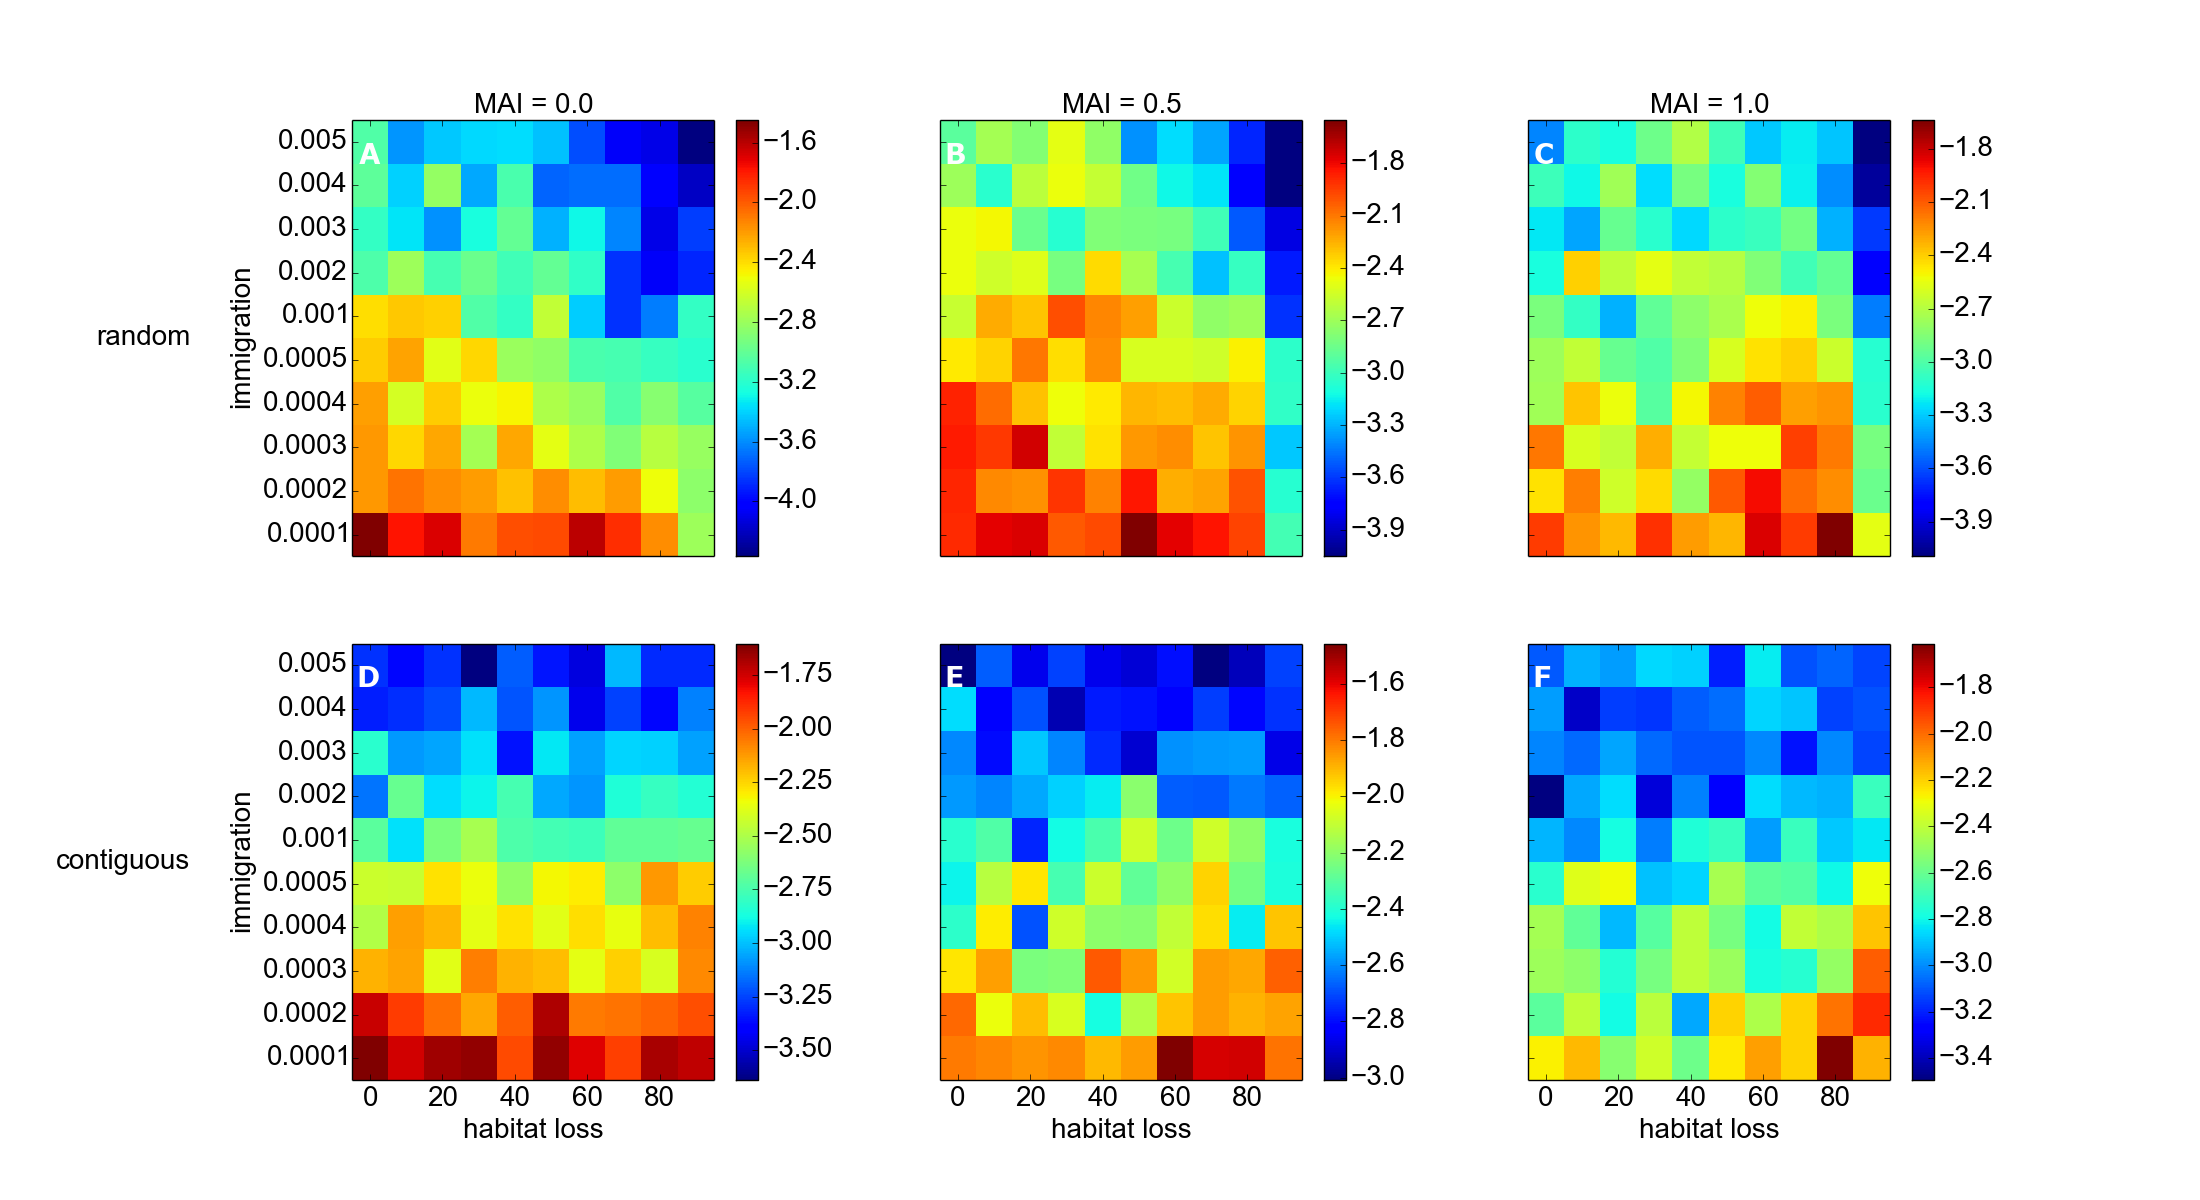
\includegraphics[width=\textwidth]{{{figures/clean_analysis/heatmap_sync}}}
	\caption{Natural logarithm of \emph{ecosystem synchrony} (ln($Sync$), defined in section \ref{sec:def_invariability} for both HL scenarios, and all three MAI ratios.}
	\label{fig:vir_sync_hm}
\end{figure}

\paragraph*{Ecosystem synchrony} (Sync) is plotted for both HL scenarios and all three MAI ratios in figure \ref{fig:vir_sync_hm}. Sync is defined in equation \eqref{eq:def_eco_sync}, and is higher when there is some degree of synchronisation between the population dynamics at the species level. The metric approaches one for perfect synchronisation (with zero phase difference)  of all species. The results shown confirm our prediction that reducing IR increases synchrony of the population dynamics, in general. From the analysis in chapter \ref{chap:stress_testing} we can now be confident that this is due to an increase in the deterministic component (due to species interactions) relative to the stochastic component (due to immigration). Less clear from this figure is the dependence of synchrony on HL. In the random scenario HL \emph{mainly} reduces synchrony, while in the contiguous scenario HL appears to \emph{mainly} have no effect on synchrony. However both of these observations are less clear at MAI$=1.0$.

\paragraph*{In summary} the results presented in this section are generally consistent with those of chapter \ref{chap:habitat_loss_high_immigration}, i.e. community responses to HL do not change when IR is varied. The notable exception to this is that at low IR random HL results in a \emph{net increase} in temporal variability, rather than a net decrease. The increase in variability occurs at high levels of HL ($>70\%$), and is most visible at HL$=90\%$ where the number of individuals is lowest. It is worth noting that the metric CV (equation \eqref{eq:cov}) tends to infinity as the number of individuals tends to zero. This property of the metric may explain the apparent increase in variability in highly impacted landscapes at low IR.

The results also confirm our prediction that reducing IR would increase the effects associated with species interactions. Temporal variability and ecosystem synchrony increase and decrease with IR respectively. Therefore the conclusion from chapter \ref{chap:stress_testing}, that reduced immigration increases the determinism and variability of population dynamics, is robust across this region of parameter space under both HL scenarios. We did not anticipate an increase in interaction strengths due to reduced IR, an effect which is present in all cases. It is not clear why reducing IR increases the mean probability of trophic interactions between species (see discussion in section \ref{sec:res_synthesis} for interpretation of IS in terms of probability). We suggest that this is again due to the limit behaviour of the metric. The metric IS (equation \eqref{eq:is3}) tends to infinity when the number of individuals belonging to one of the interacting species tends to zero. Therefore the increase in mean IS due to reduced IR may be the result of interaction strength distributions skewed by species with very low abundance.

%We suggest that it may be due to the dominance of communities by abundant and strongly interacting species. However it is also worth noting again the limit behaviour of the metric IS (equation \eqref{eq:is3}). This metric tends to infinity when the number of individuals belonging to one of the interacting species tends to zero. Therefore the increase in mean IS due to reduced IR may be the result of interaction strength distributions skewed by species with very low abundance. Both hypotheses about the unexpected change in IS are investigated in section \ref{sec:WHERE}. 

\subsection{Key points and outstanding questions}
\label{sec:questions}

%complete the section after writing up rest of chapter. 

The initial analysis of results presented in this section (\ref{sec:init_res}) highlights certain key features of community responses to varying IR and HL, which we explore further in the rest of this chapter. The aforementioned key features are as follows:

\begin{itemize}
	\item Mutualistic communities exhibit more extinctions than antagonistic communities.
	\item The total number of individuals becomes less sensitive to IR at high MAI ratios.
	%\item Mutualistic communities do not decrease in evenness at any IR, whereas antagonistic communities do*
	\item At the lowest IR values the total number of individuals increases in antagonistic communities.
	\item Contiguous HL produces more extinctions than random HL. Also, in the random scenario, the number of extinctions is less sensitive HL, especially for mutualistic communities.
	\item In certain cases the evenness of communities decrease along the HL gradient.
	%\item Why does IS increase with IR? (see two hypotheses above)
	%\item Why does variability increase (net) across the random HL gradient at low IR? (study up-tick)
	%\item How does community dependence on immigration vary?
	%\item How do network properties vary?
	%\item Is our definition of extinction OK? Which species go extinct and why? (relates to difference between contiguous and random HL)
\end{itemize}

To investigate these features further we conduct bivariate analyses similar to those in chapter \ref{chap:habitat_loss_high_immigration}. The relevant metrics are plotted against ether HL or IR, with the other variable held constant, and linear models are fitted to identify significant trends (see section \ref{sec:sampling}). To conduct the bivariate analyses we select two perpendicular transects from the region of parameter space, one at fixed IR value and one at fixed HL value. The transect at fixed IR allows use to study trends in response to HL only (section \ref{sec:biv_fixIR}), while the transect at fixed HL allows us to study trends in response to IR (section \ref{sec:biv_fixHL}). In section \ref{sec:biv_fixIR} we select a fixed IR value of $0.0005$, representing an intermediate IR at which we have observed that communities may become less even in response to HL (figures \ref{fig:vir_diversity_random_hp}, and \ref{fig:vir_diversity_contiguous_hp}). This observation indicates that community responses to HL are different at this IR value from those presented in chapter \ref{chap:habitat_loss_high_immigration}, and are therefore of particular interest. In section \ref{sec:biv_fixHL} we select a fixed HL value of $40\%$.  This represents an intermediate level of HL at which community responses may be detected (for example species extinctions at low IR), and therefore allows us to compare differences between the two HL scenarios along an IR gradient.

% can largely be extrapolated form those in the previous two chapters and confirm our predictions. There are no surprises in the contiguous case. Although we note the variability and IS responses are consistent with, and therefore support conclusions drawn from, previous analysis. Also the similarity between the results for number of interactions and number of individuals, in both HL scenarios, supports our assertion from chapter \ref{chap:habitat_loss_high_immigration} that interaction frequencies are largely driven by abundance. We did not expect to see an increase in IS as IR is reduced, an effect which is present in all cases. However we did predict that effects due to species interaction would come to play a more important role as immigration was reduced. 
%The variability response under random HL is another unexpected feature. In many instances random HL causes an initial decline, followed by a subsequent increase in temporal variability. This pattern appears robust across IRs and MAI ratios (panels C,F,I, figure \ref{fig:vir_var_random}). In fact, returning to figure \ref{fig:strong_fig} the same effect is present in our original results. The temporal variability increases at $90\%$ HL. We explore this feature further in section \ref{sec:whereis} below.
%


%% Don't necessarliy want to analyse invariability metrics:
%\begin{figure}[hb]
%	\includegraphics[width=\textwidth]{{{figures/clean_analysis/random/heatmap_inv}}}
%	\caption{Random HL. Ecosystem synchrony. Ecosystem invariability. Population invariability.}
%\end{figure}
%
%\begin{figure}[hb]
%	\includegraphics[width=\textwidth]{{{figures/clean_analysis/contiguous/heatmap_inv}}}
%	\caption{Contiguous HL. Ecosystem synchrony. Ecosystem invariability. Population invariability.}
%\end{figure}

%%%%%%%%%%%%%%%%%%%%%%%%%%%%%%%%%%%%%%%%%%%%%%%%%%%%%%%%%%%%%%%%%%%%%%%%%%%%%%%%%%%%%%%%%%%%%%%%%%%%%%%%%%%%%5
%% For now we do not look gere at dependence on immigration..maybe later?
%\subsection{Dependence on immigration}
%\label{sec:dependence_on_im}
%
%%% This figure produce by: /MyFiles/cm1788/Documents/IM_vs_HL_heatmap/clean_results/random/plot_immap.py
%%% Might need to re-scale if colours not clear when printed?
%\begin{figure}[hb]
%	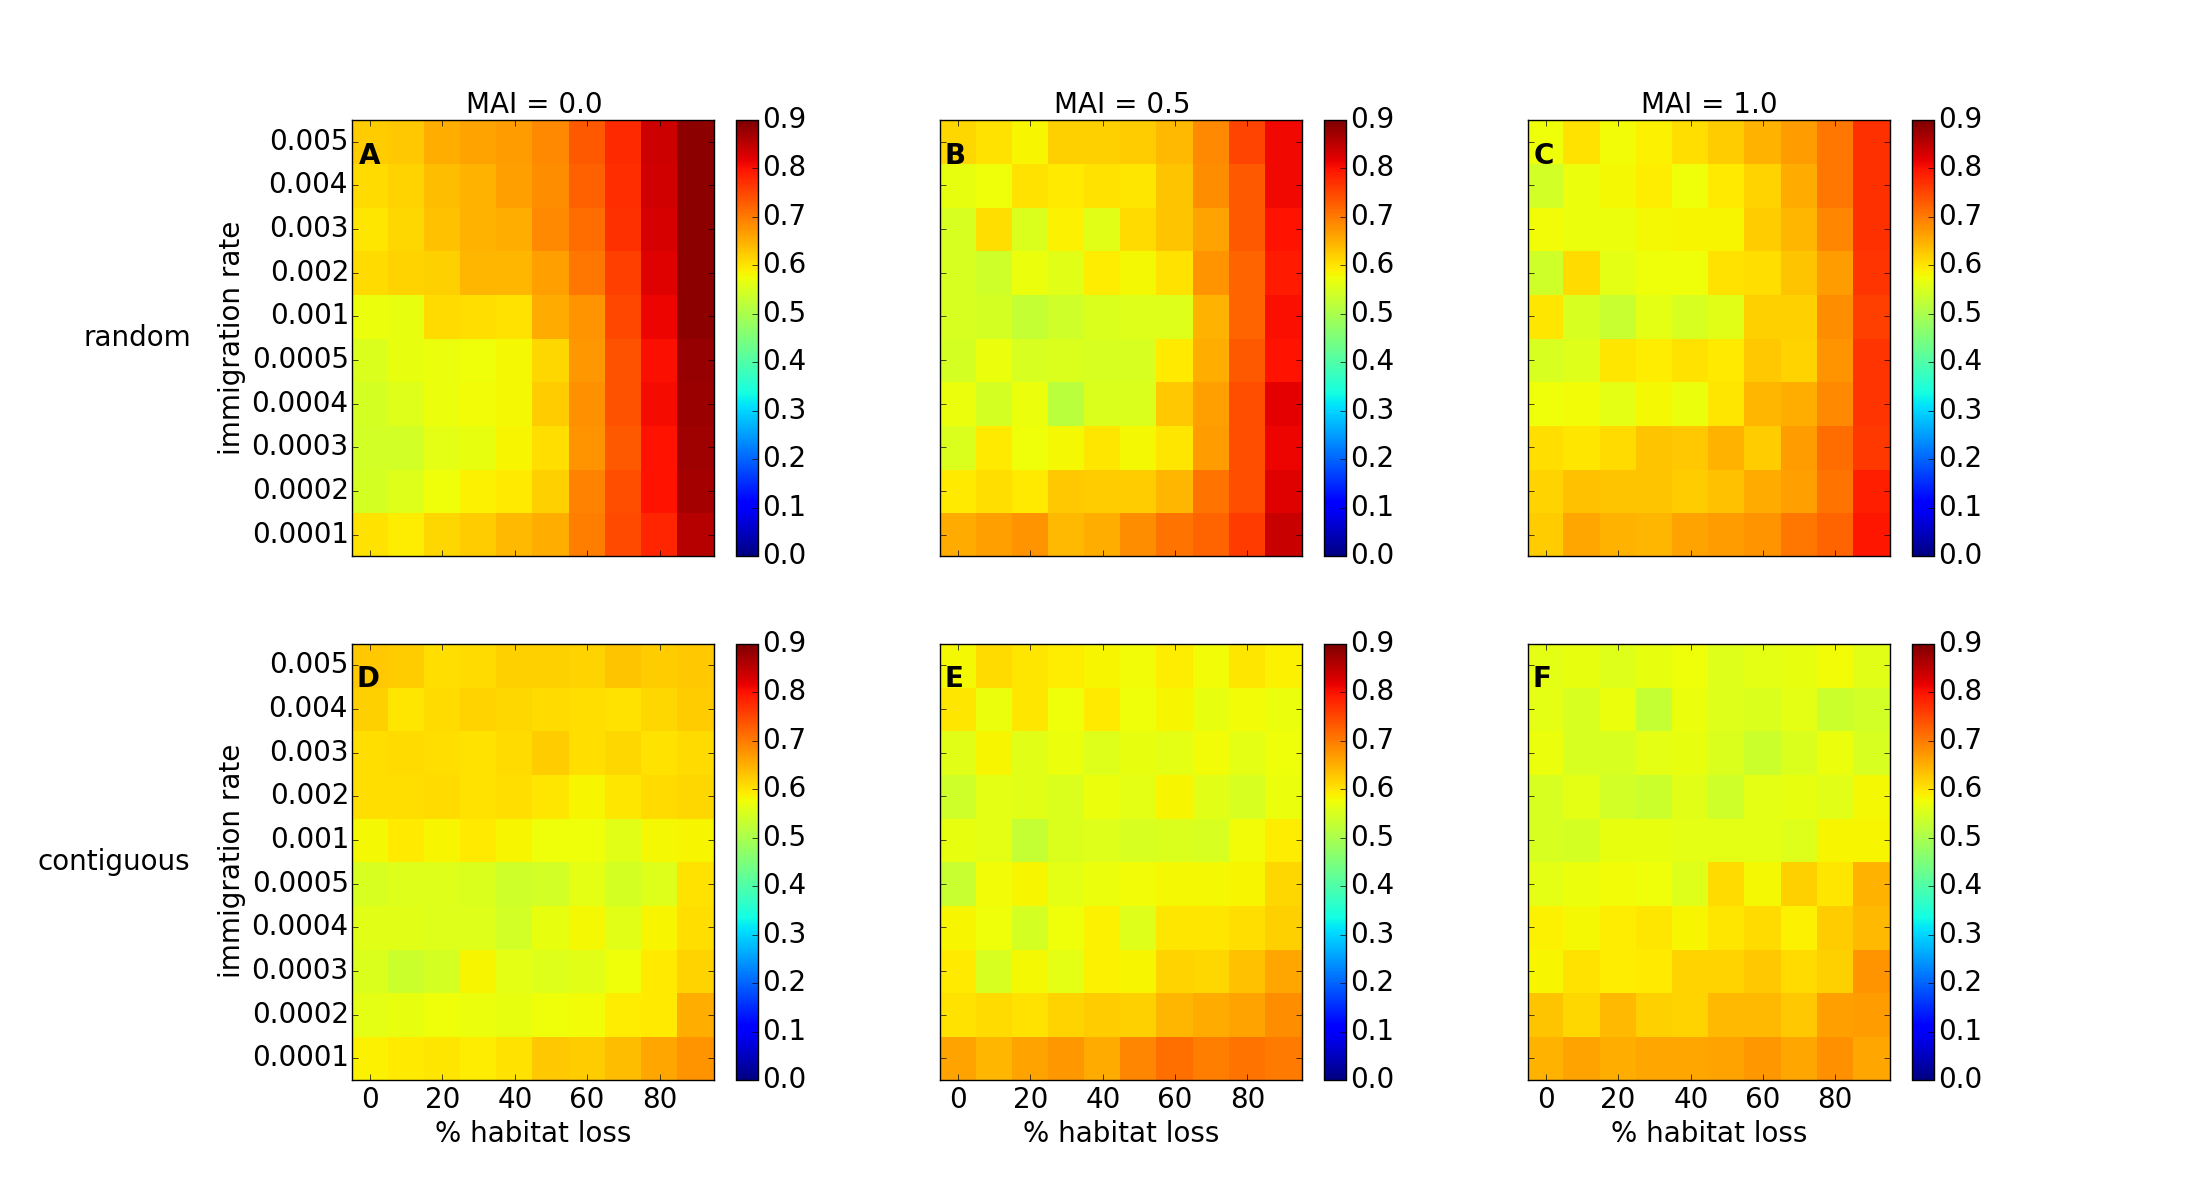
\includegraphics[width=\textwidth]{{{figures/clean_analysis/heatmap_proportion_im}}}
%	\caption{Similar to figure \ref{fig:vir_sync_hm}, but displaying the proportion of the total number of individuals born that come from immigration, calculated as in figure \ref{fig:res_proportion_immigrants}.}
%	\label{fig:proportion_im_heatmap}
%\end{figure}
%%%%%%%%%%%%%%%%%%%%%%%%%%%%%%%%%%%%%%%%%%%%%%%%%%%%%%%%%%%%%%%%%%%%%%%%%%%%%%%%%%%%%%%%%%%%%%%%%%%%%%%%%%%%%%

\section{Bivariate analysis: fixed IR}
\label{sec:biv_fixIR}

%\begin{itemize}
%	\item Differential response of mutualistic and antagonistic communities - needs investigating. Community composition, esp MAI ratios under changing IR.
%	\item Do communities really become less even at some IRs (bivariate analysis), and is this associated by a reduced dependence on immigration...
%	\item Why does abundance suddenly increase at low IR in antagonistic communities?
%	\item Why does contiguous HL generate more extinctions? And why are extinctions not dependent on HL in the random case?
%	\item Why does IS increase as IR reduced? Dominant species? Check distribtuions..
%	\item What is going on with variability in the random scenario? (Does new metric meancv\_sqaured solve it?)
%	\item Proportion of immigration not as as simple as expected..
%\end{itemize}

%CHANGE THIS: In this section we look in more detail at the results summarised in section \ref{sec:init_res} by conducting bivariate analysis of certain key metrics, as we did in chapter \ref{chap:habitat_loss_high_immigration}. From the depiction of how metrics vary across the slice of parameter space we select an immigration rate (IR) of $0.0005$ at which to study the response of communities to HL. 

Here we study community response to HL at IR$=0.0005$. This IR is an order of magnitude below the \emph{default value} of $0.005$ used in chapter \ref{chap:habitat_loss_high_immigration}. Therefore some significant differences in community response are expected, and are anticipated from the results of section \ref{sec:init_res} as discussed above.

%The choice of such an IR here is justified by..We focus on evenness..and community composition..extinctions later?

\subsection{Evenness}
\label{sec:biv_HL_evenness}

\begin{figure}
	\centering	
	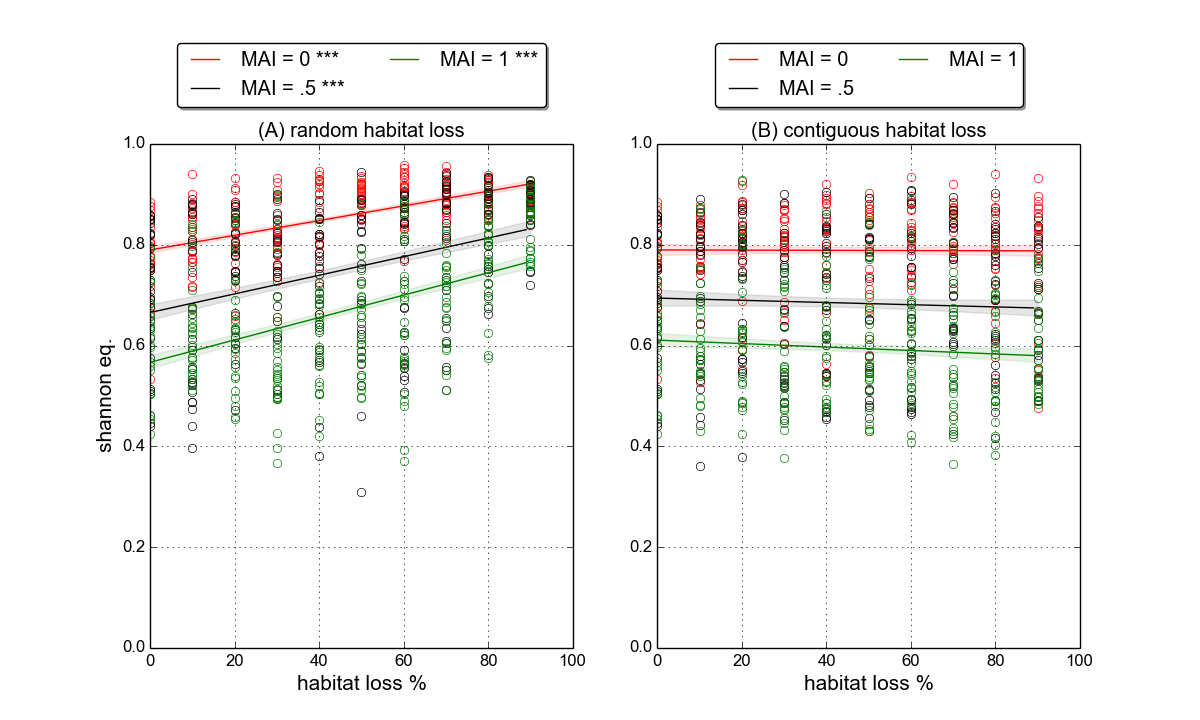
\includegraphics[width=\textwidth]{{{figures/bivariate_v_HL/clean_lm_shannon_eq_3mai}}}
	\caption{\textbf{Shannon equitability} against percentage habitat loss, for both scenarios: (A) Random HL, and (B) Contiguous HL. The format of these bivariate plots is standardised, and consistent with those in chapter \ref{chap:habitat_loss_high_immigration}. Circles represent the metric value for a single community; lines represent a linear fit to the data and the shaded regions indicate the standard error of the mean. The markers ***, **, * and + corresponds to linear model fit p-values of $<0.001$, $<0.01$, $<0.05$ and $<0.1$ (marginal significance) respectively.}
	\label{fig:biv_HL_shannon_eq}
\end{figure}

Figure \ref{fig:biv_HL_shannon_eq} shows how the \emph{Shannon equitability} metric, calculated at the community level, changes across the HL gradient under both HL scenarios. This metric (equation \eqref{eq:shan_eq}) measures how evenly abundance is distributed between all species present in the community. Maximum evenness is achieved when all species have the same abundance, in which case the metric is equal to one. From the figure we see a characteristic feature of the model, that low MAI communities are more even than high MAI communities (previously explained in chapter \ref{chap:habitat_loss_high_immigration} and \cite{lurgi2015effects}). We also observe from the figure that communities in pristine landscape have similar evenness as those simulated with the default IR value (compare to figure \ref{fig:shannon_eq}). This similarity is surprising given that we have argued previously that immigration drives evenness, and that here the magnitude of IR is an order of magnitude lower than the default value. The linear models confirm the trends in evenness, observed in section \ref{sec:vir_diversity}, that inspired this choice of IR value to study. Under both types of HL antagonistic communities (MAI$=0.0$) \emph{become significantly less even}. Communities at intermediate MAI ratio ($0.5$) do not become significantly more or less even under either type of HL, while high MAI communities ($1.0$) respond in opposite directions. At MAI$=1.0$ communities become more even and less even under random and contiguous HL respectively, although the p-value and the slope of the trend is lower in the contiguous case. The observation that varying the level of mutualism can change the qualitative response of communities to HL is novel to this chapter.

%This is a new observation, which we seek to explain below\footnote{HOw?}

The evenness responses are explored further by calculating the Shannon equitability within each trophic level. These results are shown in figure \ref{fig:biv_HL_shannon_eq_TL} for both HL scenarios. The plots reveal that there is a difference between the  equitability response at the community level compared to that within trophic levels, especially under random HL. In the random scenario (panels A,C,E,G) the distribution of abundances within all trophic levels becomes more even, except for the top trophic level of antagonistic communities (MAI$=0.0$, panel G). Therefore antagonistic communities become less even on aggregate, but more even within three out of the four trophic levels. Communities at intermediate MAI ratio ($0.5$) become more even within all trophic levels but do not change on aggregate, whereas high MAI communities ($1.0$) become more every at every level. In the contiguous scenario antagonistic communities  become less even within trophic levels, which is consistent with the community level response. Mutualistic communities (MAI$=0.5,1.0$) do not exhibit changes in evenness within any trophic level. For MAI$=0.5$ this is consistent with the community level, but for MAI$=1.0$ community level evenness decreases despite constant evenness within the trophic levels.   


\begin{figure}
	\centering	
	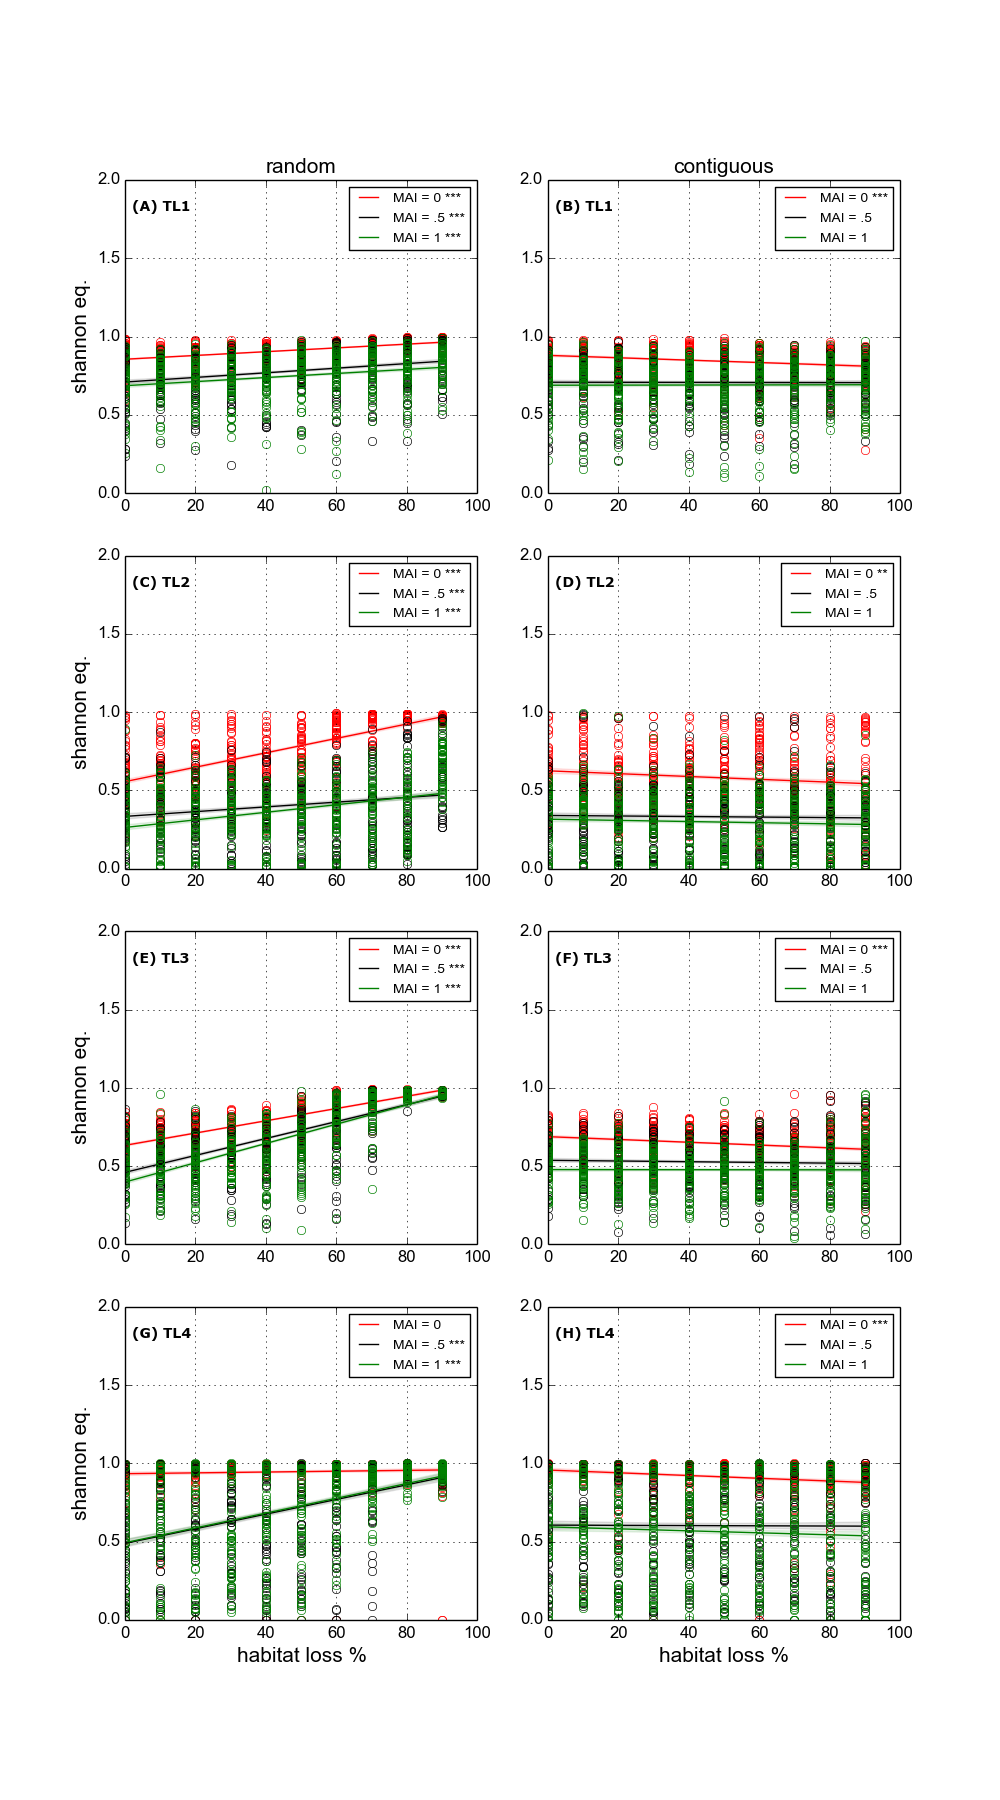
\includegraphics[width=0.7\textwidth]{{{figures/bivariate_v_HL/lm_fg_shannon_eq_hl_contiguous_3mai}}}
	\caption{\textbf{Shannon equitability} against percentage habitat loss, for each trophic level. Left column: random HL. Right column: contiguous HL. Format of individual plots is the same as in figure \ref{fig:biv_HL_shannon_eq}.}
	\label{fig:biv_HL_shannon_eq_TL}
\end{figure}


\subsection{Rank-abundance distributions}
\label{sec:biv_HL_RADs}

In this section we present rank-abundance distributions (RADs) for example communities. Each RAD plotted is for single community selected from the 50 replicates to characterise the general features of the distributions at given HL values and MAI ratios. Together the RADs help to explain the observed evenness responses from section \ref{sec:biv_HL_evenness}, especially the discrepancy between some community level and trophic level responses. In some cases the RADs contain discontinuities (for example figure \ref{fig:biv_HL_rads_mai0_random},panel C). The \emph{Zipf} and \emph{pre-emption} model fits to the RADs, illustrated in the plots as solid red and blue lines respectively, are unable to characterise the discontinuities. Therefore the fitted model parameters (alpha and gamma) are not used as complementary measures of community evenness, as they were in chapter \ref{chap:habitat_loss_high_immigration}.

\begin{figure}
	\centering	
	\includegraphics[width=\textwidth]{{{figures/bivariate_v_HL/example_RADS_mai0_random}}}
	\caption{\textbf{Example rank-abundance distributions} (RADs) for three \textbf{antagonistic communities} (MAI$=0.0$), under \textbf{random HL}, at \textbf{IR}$\mathbf{=0.0005}$. (A) HL=$0\%$, (B) HL=$50\%$, (C) HL=$90\%$. Species abundances are relative to the total number of individuals in the community, and plotted on a logarithmic scale. Circles represent species, coloured according to trophic level: green=basal; blue=herbivore/animal-mutualist; yellow=primary predator; red=top predator. Blue and red lines give the pre-emption and Zipf model fits respectively (see text in section \ref{sec:define_rads} for definitions), best fit parameter value for each model given as annotations on plot.}
	\label{fig:biv_HL_rads_mai0_random}
\end{figure}

Figure \ref{fig:biv_HL_rads_mai0_random} shows RADs for antagonistic communities (MAI$=0.0$) under random HL. Such communities were observed (section \ref{sec:vir_diversity}) to become less even at the community level, but more even within trophic levels, in response to HL. Comparing panels A and C it is clear that the decrease in community level evenness is due to an increased dominance of plant species. The RAD at at HL$=90\%$ is dominated by 16 plant species, with all other species having a relative abundance of less than 0.01. The discontinuity observed here, between the groups of most and least abundant species, is characteristic of communities under random HL at this value of IR. This observation leads us to define the terms \emph{core} and \emph{tail} to refer to the two groups of relatively high and low abundance species. In what follows we use 0.01 as the threshold relative abundance that separates the two groups. The core and tail sections of the RAD at HL$=90\%$ are relatively even when considered separately. Therefore the increased evenness within trophic levels one, two and three follows intuitively. In the RAD at HL$=0\%$ species belonging to these three trophic levels are interspersed along the distribution, whereas at HL$=90\%$ each trophic level is contained within either the core or tail section only\footnote{`trophic sorting'?}.

%% Not sure about this plot: interesting, but may confuse the message, just see example RADs
%\begin{figure}
%	\centering	
%	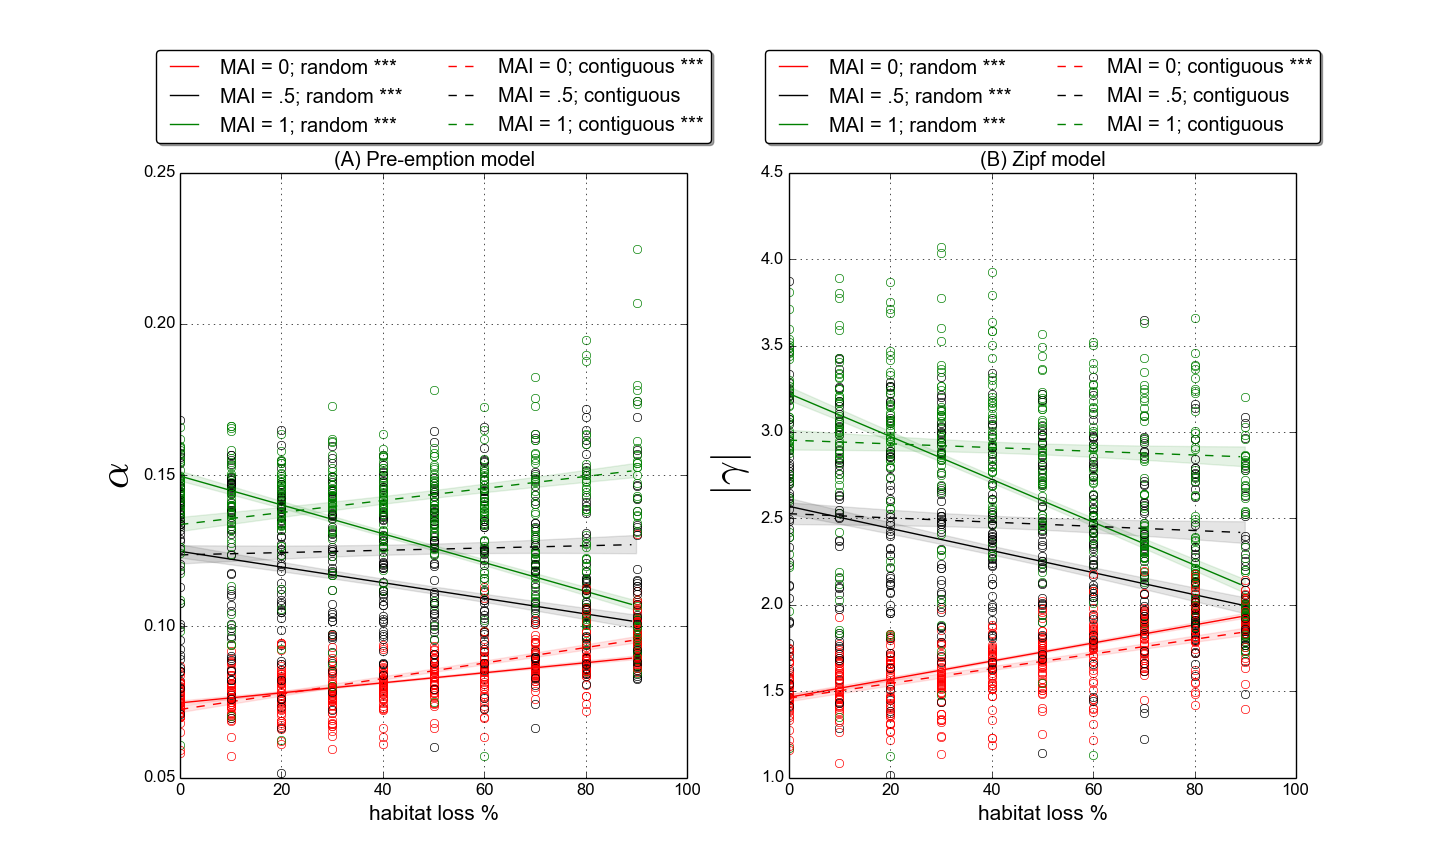
\includegraphics[width=\textwidth]{{{figures/bivariate_v_HL/lm_radfit_params_v_hl}}}
%	\caption{\textbf{Rank abundance model fit} parameters against HL. Panel A: Pre-emption model parameter $\alpha$ is smaller for more even distributions. Panel B: Absolute value of Zipf model parameter $\left| \gamma \right|$ is smaller for more even distributions. (See model definitions in section \ref{sec:define_rads}). Solid lines represent linear fits to the random HL data, dashed lines indicate linear fits to the contiguous HL data, and error bars give $\pm 1$ standard-deviation. *** indicates p-value $<0.001$ for linear model fit, whilst no marker indicates p-value$>0.1$.}
%	\label{fig:biv_HL_radfit}
%\end{figure}

\begin{figure}
	\centering	
	\includegraphics[width=\textwidth]{{{figures/bivariate_v_HL/example_RADS_mai1_random}}}
	\caption{Similar to figure \ref{fig:biv_HL_rads_mai0_random}, but for \textbf{mutualistic communities} (MAI$=1.0$), under \textbf{random HL}.}
	\label{fig:biv_HL_rads_mai1_random}
\end{figure}

Figure \ref{fig:biv_HL_rads_mai1_random} shows RADs for mutualistic communities (MAI$=1.0$) under random HL. Such communities were observed (section \ref{sec:vir_diversity}) to become more even at the community level, and within all trophic levels, in response to HL. Here the role of mutualism in reducing community evenness is very clear. In pristine habitat (panel A) the community is uneven with a core of ten abundant species. The difference between this mutualistic community and the equivalent antagonistic one (\ref{fig:biv_HL_rads_mai0_random}, panel A) is striking. Here the dominance of the core species must be due to the benefit of mutualism, which is not solely conferred on species that interact mutualistically (i.e. plant and animal mutualists). The core contains species belonging to all trophic levels. In agreement with our observations at zero IR (chapter \ref{chap:stress_testing}) some species in higher trophic levels, presumably those feeding on mutualists, benefit from the presence of mutualism in the community. However other species appear to suffer as a result of the increased fitness of their competitors. These species form a tail of low abundance resulting in a very uneven community. In fact 15 species are totally extinct (zero individuals) from this community, in a landscape without HL. Increasing HL to $50\%$ (panel B) creates a flatter distribution with no clear distinction between core and tail, and no extinct species. The result that increasing random HL can reduce extinctions at MAI$=1.0$ is present in some but not all replicate communities at this IR value. At HL$=90\%$ (panel C) the RAD is more even than at $0\%$, although there is once again a discontinuity between core and tail. In this instance the core consists of only species belonging to trophic levels one and two. This suggests that, in highly impacted random landscapes, mutualistic-animals may still benefit directly from their mutualistic interactions, but that this benefit is no longer passed up the food chains.

\begin{figure}
	\centering	
	\includegraphics[width=\textwidth]{{{figures/bivariate_v_HL/example_RADS_mai0_contiguous}}}
	\caption{Similar to figure \ref{fig:biv_HL_rads_mai0_random}, but for \textbf{antagonistic communities} (MAI$=0.0$), under \textbf{contiguous HL}.}
	\label{fig:biv_HL_rads_mai0_contiguous}
\end{figure}

Figure \ref{fig:biv_HL_rads_mai0_contiguous} shows RADs for antagonistic communities (MAI$=0.0$) under contiguous HL. Such communities were observed (section \ref{sec:vir_diversity}) to become less even on average at both the community level and within trophic levels. Panel A is a replicate community corresponding to the same panel of figure \ref{fig:biv_HL_rads_mai0_random}, since HL$=0\%$ in both cases. The RADs are qualitatively similar. From figure \ref{fig:biv_HL_rads_mai0_contiguous} the communities do appear to become less even along the contiguous HL gradient. HL is also seen to cause extinctions, which we know from figure \ref{fig:vir_diversity_contiguous_hp} is a general feature of the contiguous scenario at this IR. At $90\%$ HL two species have an absolute abundance of zero, while a number of other species have low relative abundances in discrete steps (presumably corresponding to absolute abundances of one,two, three, individuals, etc.). This pattern suggests that many species are on the border of total extinction in this community, as predicted in section \ref{sec:motivate_immigration}. However the discontinuity that was characteristic of RADs in the random scenario is not present, such that there is no clear distinction between core and tail species (in such cases the \emph{Zipf} and \emph{preemption} model coefficients may be used to quantify evenness).
%
%\begin{itemize}
%	\item Relatively even in pristine landscape, like figure \ref{fig:biv_HL_rads_mai0_random}.
%	\item Becomes slightly less even at community and trophic levels. 
%	\item However the discontinuity characteristic of the random scenario is not present. Presumably in the contiguous case these rare species are still able to interact, therefore reproduce and feed, and are fed upon.
%\end{itemize}

\begin{figure}
	\centering	
	\includegraphics[width=\textwidth]{{{figures/bivariate_v_HL/example_RADS_mai1_contiguous}}}
	\caption{Similar to figure \ref{fig:biv_HL_rads_mai0_random}, but for \textbf{mutualistic communities} (MAI$=1.0$), under \textbf{contiguous HL}.}
	\label{fig:biv_HL_rads_mai1_contiguous}
\end{figure}

Figure \ref{fig:biv_HL_rads_mai1_contiguous} shows RADs for mutualistic communities (MAI$=1.0$) under contiguous HL. Such communities were observed (section \ref{sec:vir_diversity}) to become slightly less even on average at the community level, but the evenness did not change significantly within functional groups. Panel A is a replicate of the community in the same panel of figure \ref{fig:biv_HL_rads_mai1_random}, since HL$=0\%$ in both cases. In figure \ref{fig:biv_HL_rads_mai1_contiguous} there is less of a distinction between core and tail, and there are fewer extinct species, but otherwise the RADs are qualitatively similar. These mutualistic communities are less even than the antagonistic communities in figure \ref{fig:biv_HL_rads_mai0_contiguous} because of the effect of mutualism already discussed. The communities also decrease in evenness along the HL gradient, and exhibit more species extinctions than the antagonistic equivalents.  We suggest that the reason evenness does not decrease within trophic levels due to HL, is partly that these communities already have low evenness in pristine landscape. A wide range of relative abundances for all four trophic levels is visible in panel A of the figure. Once again there is not a clear discontinuity between core and tail species. However at $90\%$ HL the tail-end of the distribution again displays discrete steps in relative abundances characteristic of species on the border of extinction.

A NOTE HERE ON WHAT THE RADS TELL US ABOUT EXTINCTIONS? (can refer forwards to here form section 5.3.1)

%\begin{itemize}
%	\item Less even in pristine landscape, although discontinuity not extreme in this community.
%	\item Becomes slightly less even at community and trophic levels. 
%	\item No clear change in evenness due to HL.
%	\item Again do distinct `tail' of low abundance species, as in the random scenario.
%\end{itemize}



\subsection{Relative abundance by functional group}
\label{sec:biv_HL_RAFG}

\begin{figure}
	\centering	
	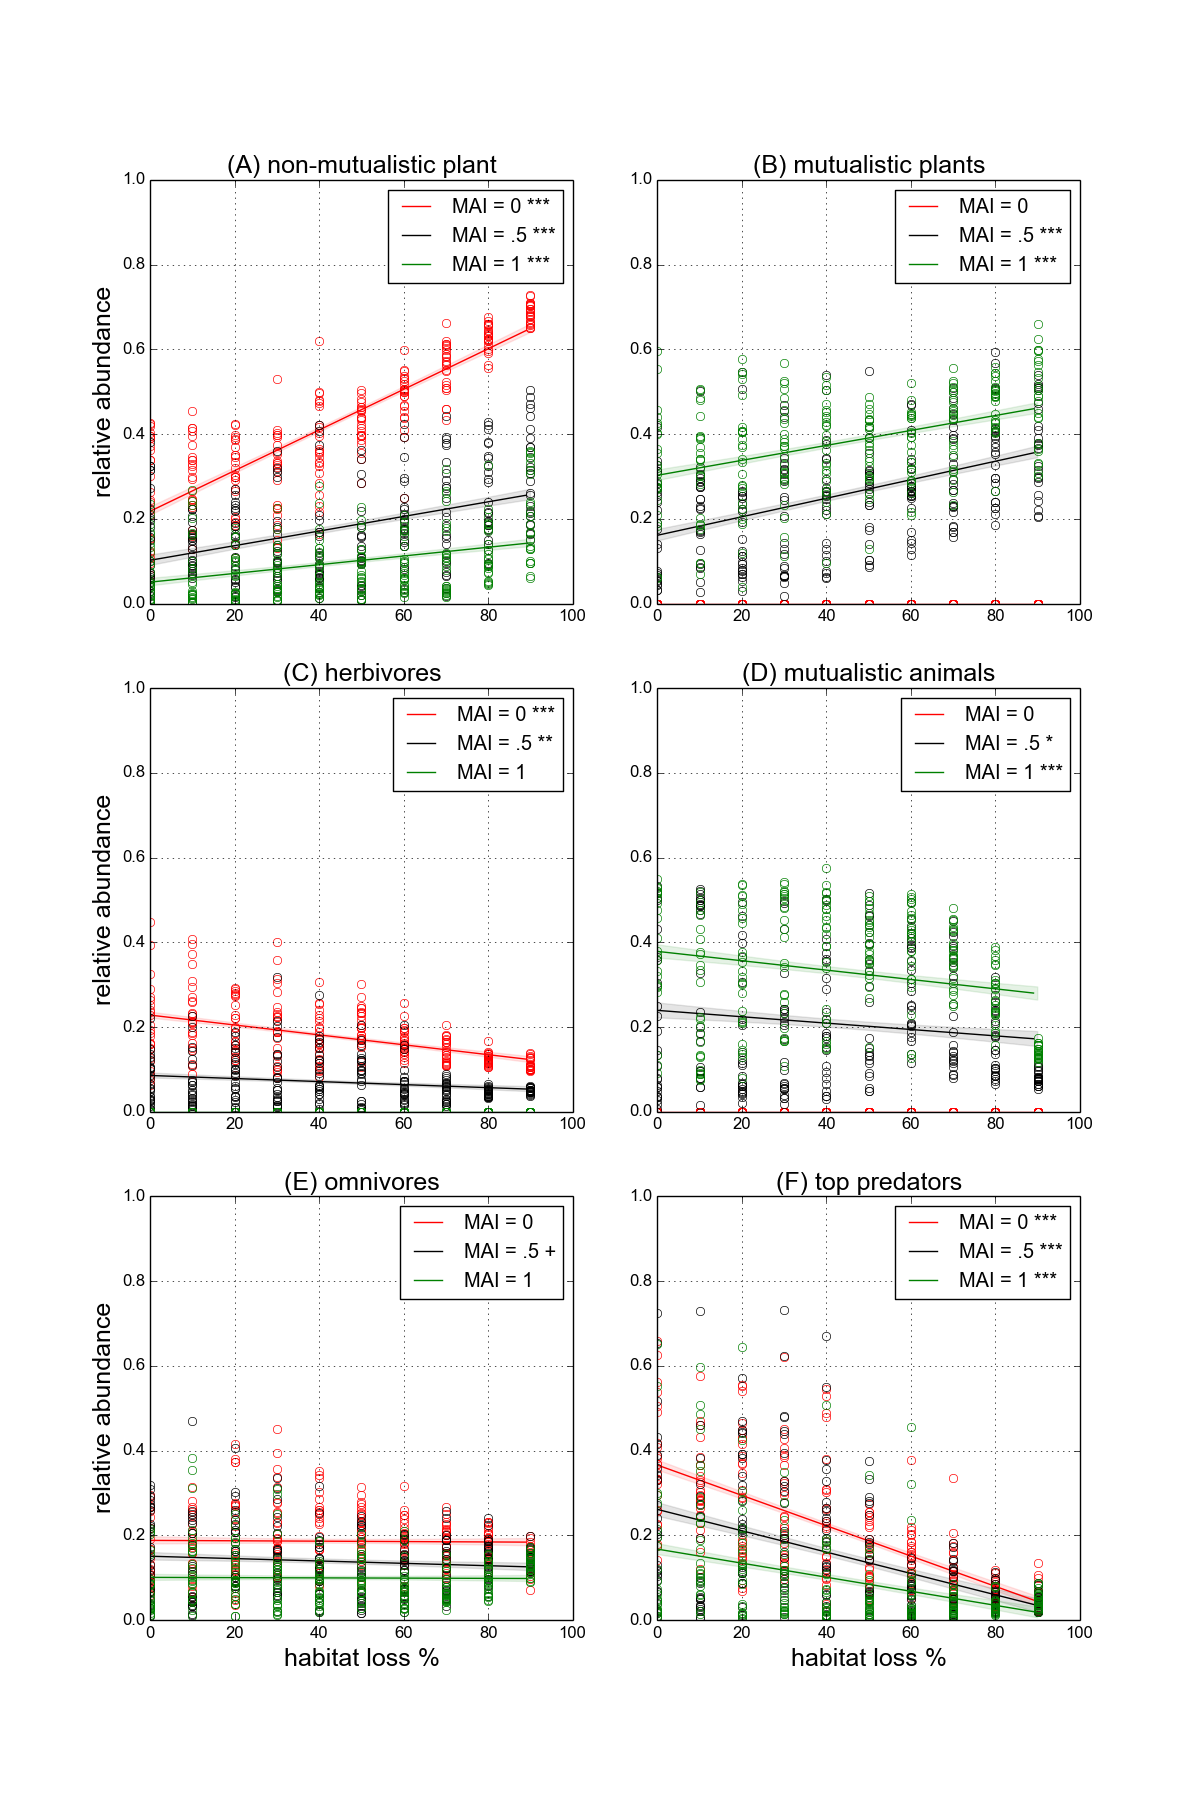
\includegraphics[width=0.8\textwidth]{{{figures/bivariate_v_HL/lm_fg_relative_abundance_hl_random_3mai}}}
	\caption{\textbf{Relative abundance} by functional group for \textbf{random HL}. Abundance relative to total number of individuals in the community. Format of individual plots is the same as in figure \ref{fig:biv_HL_shannon_eq}.}
	\label{fig:biv_HL_proportion_by_fg_random}
\end{figure}

In this section we briefly consider how the relative abundance of the functional groups responds to HL at the same IR value (0.0005). Figure \ref{fig:biv_HL_proportion_by_fg_random} shows the relative abundance of each functional group under random HL. The main feature of these plots is that random HL causes a shift in biomass towards the basal trophic level. The same type of shift was observed at the default IR value in chapter \ref{chap:habitat_loss_high_immigration}, however it is more extreme at this low IR. The only non-basal functional group which retains any appreciable abundance up to high levels of HL ($90\%$) are mutualistic-animals. At $90\%$ HL antagonistic communities become almost completely dominated by plants (relative abundance $<0.9$), while communities with mutualism become dominated by plants (mutualistic and non-mutualistic) and mutualistic-animals. Both these observations are consistent with the RADs presented in section \ref{sec:biv_HL_RADs}. The shift towards basal species under random HL is due to weaker trophic interactions, which in turn is related to the decreased mobility of individuals in a randomly impacted landscape (as argued in section \ref{sec:res_synthesis}). 

At the default IR value we saw that the relative abundance of primary-predators was constant along the random HL gradient. This, it was argued, is because primary-predators are the largest functional group in terms of species and therefore receive the most input from immigration. Here we see that the relative abundance of primary-predators decreases, and we associate this difference with reduced input from immigration due to the low IR value. Also figure \ref{fig:biv_HL_proportion_by_fg_random} reveals that in pristine landscape top-predators have a lower relative abundance than at the default IR value, while plants have a higher relative abundance (especially at MAI$=0.0$, see figure \ref{fig:rel_abun_random} for comparison). We conclude that this difference is partly due to the removal of feeding links between top-predators and basal species, links which were not removed in chapter \ref{chap:habitat_loss_high_immigration}. However there may also be an effect of reduced IR. Since immigration provides a food source for all non-basal species, the reduction of IR will affect species at the top of food chain the most, whilst the reduced predation pressure will benefit basal species which do not require food.
%
%\begin{itemize}
%	\item Top predator much lower in abundance than with default IR, even in pristine landscape. Partly due to removal of feeding links. Also due to lower IR - less food available, hits this group hardest?
%	\item Basal species benefit, relatively, from random HL - reduced predation pressure
%	\item All other functional groups suffer - same reasoning given in first chapter: less feeding, less mating.
%	\item Plant come to dominate antagonistic communities at more than 0.9 RA. This explains the loss of evenness at the community level - it is due to the differential response of plant and other FGs.
%	\item In mutualistic communities, although plant abundance increase relative to other groups they do not totally dominate - combined both types of plant is about 0.7 at MAI=$1.0$. This is because mutualistic animals retain their abundance quite well - about 0.3 and MAI$=1.0$. This partly explains why evenness response is different in mutualistic communities.
%	\item Although RAs fall very low under random HL, this does not translate into extinctions,as we saw.
%\end{itemize}

\begin{figure}
	\centering	
	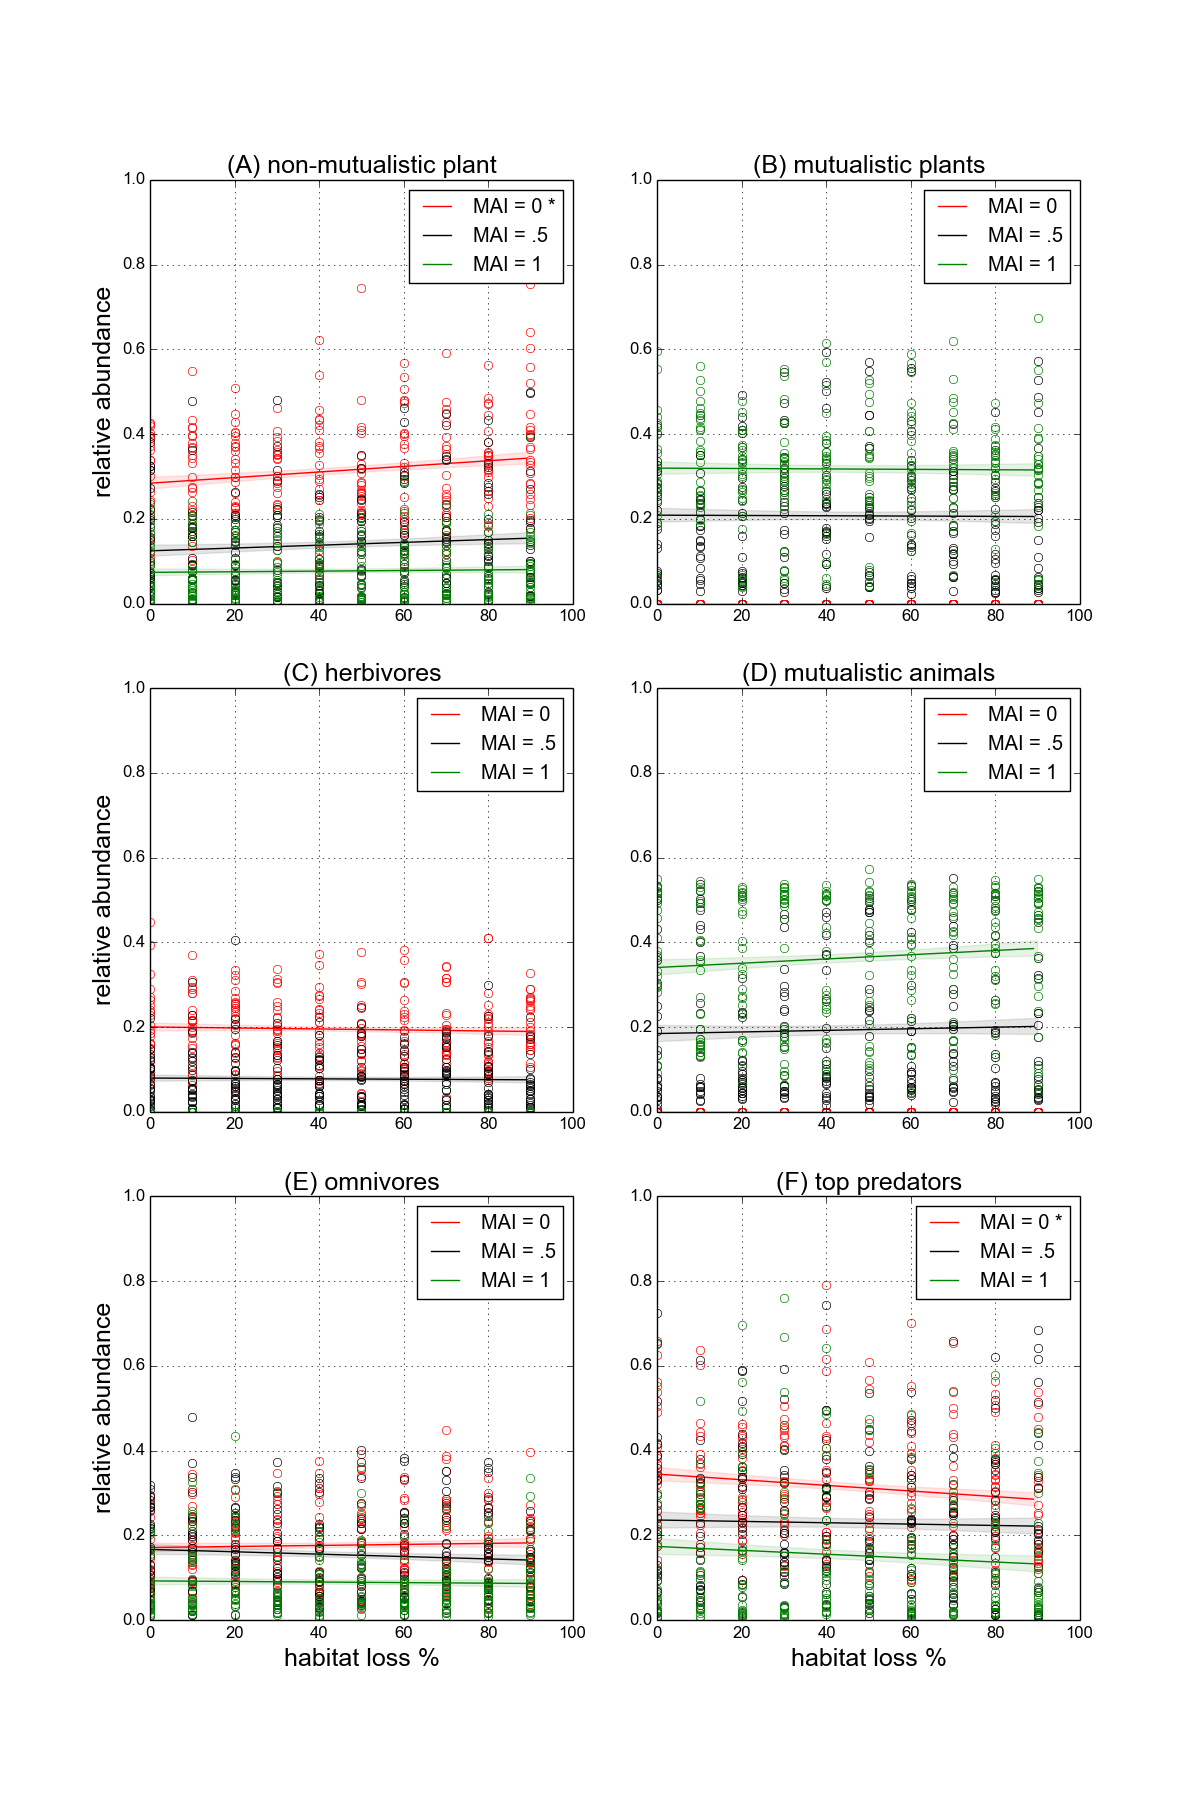
\includegraphics[width=0.8\textwidth]{{{figures/bivariate_v_HL/lm_fg_relative_abundance_hl_contiguous_3mai}}}
	\caption{\textbf{Relative abundance} by functional group for \textbf{contiguous HL}. Abundance relative to total number of individuals in the community. Format of individual plots is the same as in figure \ref{fig:biv_HL_shannon_eq}.}
	\label{fig:biv_HL_proportion_by_fg_contiguous}
\end{figure}

Figure \ref{fig:biv_HL_proportion_by_fg_contiguous} shows the relative abundance of each functional group under contiguous HL. There is a slight decrease in the relative abundance of both predator groups at all MAI ratios (panels E and F). We know that mobility (section \ref{sec:res_synthesis}) and trophic interactions (figure \ref{fig:vir_var_contiguous}) remain strong under contiguous HL. Despite this predator species suffer as a result of contiguous HL at this IR value, suggesting reduced resource availability and perhaps increased competition. At MAI$=0.0$ and $0.5$ there is an increase in the relative abundance of non-mutualistic plants, presumably due to decline in the abundance (or extinctions of) grazing species. However mutualistic-plants do not benefit, perhaps because they are grazed on by mutualistic-animals which either remain relatively abundant (MAI$=0.5$) or increase in relative abundance (MAI$=1.0$).
%
%\begin{itemize}
%	\item Slight decrease in both predator groups. Realistic. But why, when trophic interaction remain strong?
%	\item Increase in non-mutualistic plants - reduced predation??
%	\item Increase in mutualistic animals at MAI$=1.0$ - reduced predation while plant resource remains strong. But why no benefit other groups?
%	\item Otherwise first two trophic level pretty constant (as in first chapter)
%	\item These patterns hard to explain. Also relate to extinctions??
%\end{itemize}




\subsection{Network properties}
\label{sec:biv_netprops}

\begin{figure}
	\centering	
	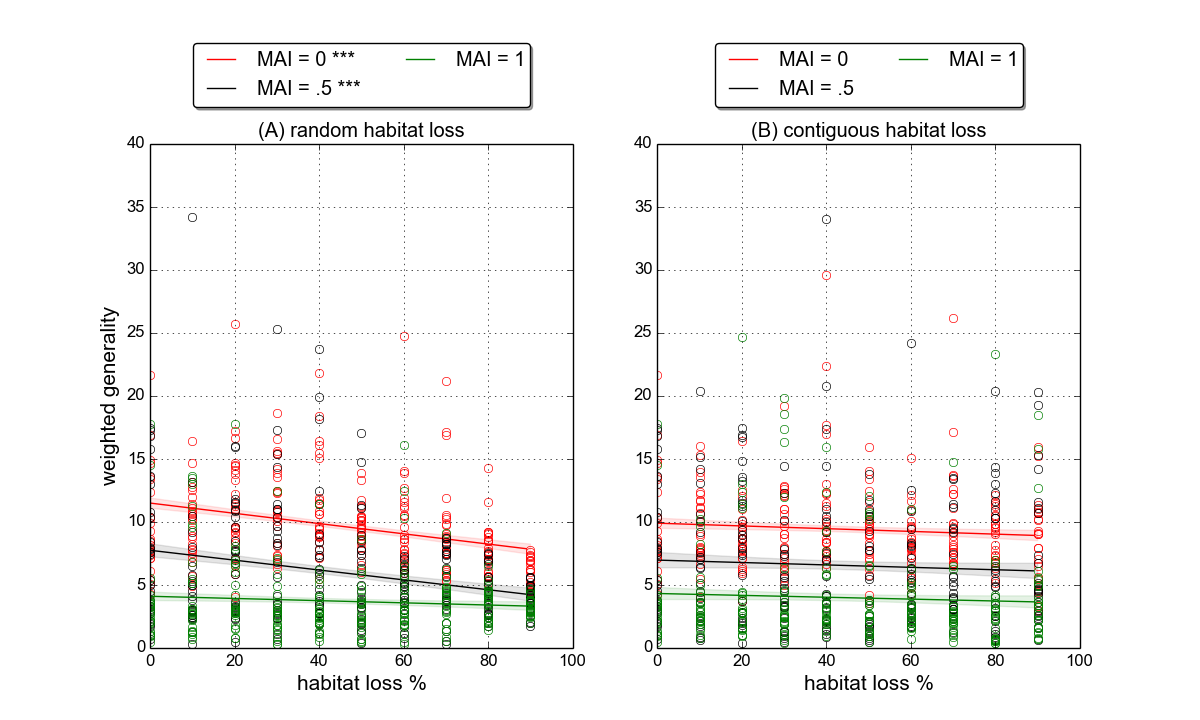
\includegraphics[width=\textwidth]{{{figures/bivariate_v_HL/clean_lm_weighted_generality_3mai}}}
	\caption{Similar to figure \ref{fig:biv_HL_shannon_eq}, but for \emph{weighted quantitative generality} (defined in section \ref{sec:define_network_metrics}). \textbf{IR}$\mathbf{=0.0005}$.}
	\label{fig:biv_HL_gen}
\end{figure}
\begin{figure}
	\centering	
	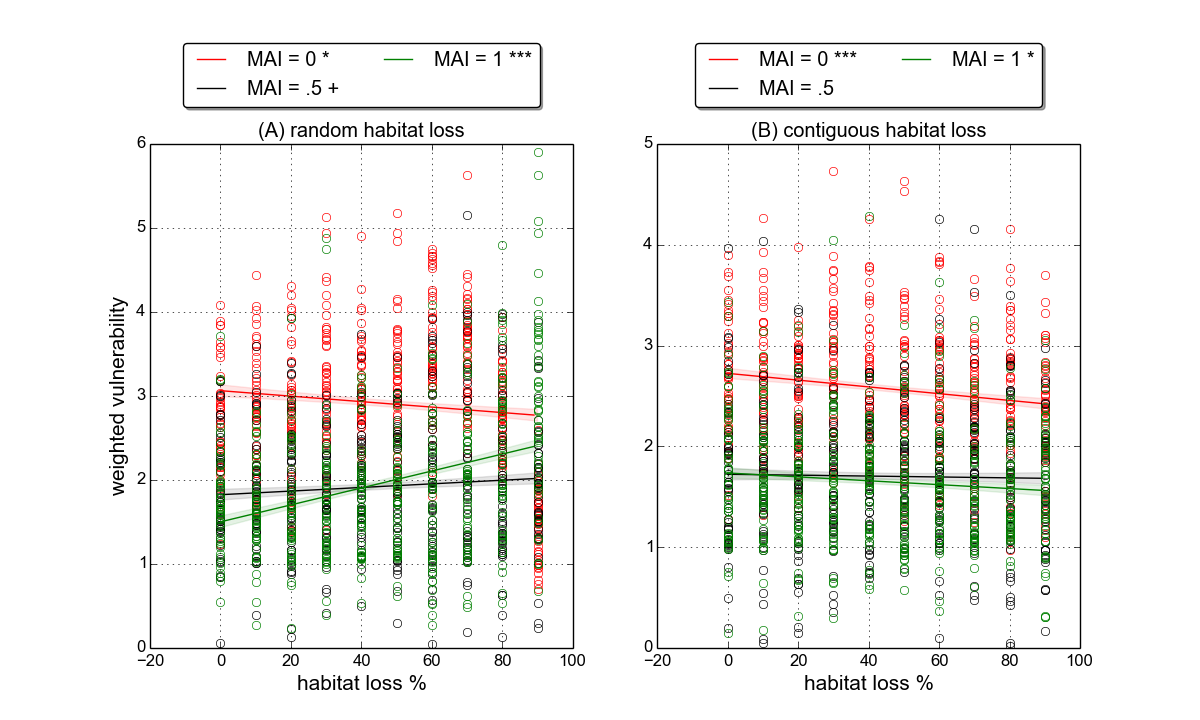
\includegraphics[width=\textwidth]{{{figures/bivariate_v_HL/clean_lm_weighted_vulnerability_3mai}}}
	\caption{Similar to figure \ref{fig:biv_HL_shannon_eq}, but for \emph{weighted quantitative vulnerability} (defined in section \ref{sec:define_network_metrics}). \textbf{IR}$\mathbf{=0.0005}$.}
	\label{fig:biv_HL_vul}
\end{figure}

We now consider changes in network properties in response to HL. For simplicity results are only presented for quantitative generality and vulnerability (defined in section \ref{sec:define_network_metrics}). In chapter \ref{chap:habitat_loss_high_immigration} we saw that the response of these metrics was associated with changes in the evenness of species abundances, or lack thereof. Therefore we may expect responses that correspond to the changes in evenness discussed in section \ref{sec:biv_HL_evenness}. However the lower IR used here (0.0005) produces species extinctions, as we have seen. The loss of species may also drive changes in network properties.

Figure \ref{fig:biv_HL_gen} shows the response of generality under random and contiguous HL. We see that generality decrease significantly in all cases, except at MAI$=1.0$ under random HL. In general the change in generality is less for communities with mutualism, and they tend to have lower generality than antagonistic communities across the HL gradient. This difference relates to the lower evenness of mutualistic communities. A decrease in the generality metric corresponds to a drop in the \emph{number of effective prey per predator}, which may be associated with a reduced number of \emph{actual} prey, a reduced evenness in interaction frequencies, or both. In the random scenario we expect a drop in the actual number of prey because of the restriction on mobility presented by destroyed cells. In the contiguous scenario a drop in the actual number of prey may be produced by species extinctions or extreme scarcity. Also in some cases at this IR value we have seen that communities become less even, which acts to reduce the evenness of interaction frequencies.

Figure \ref{fig:biv_HL_vul} shows the response of vulnerability under random and contiguous HL. A decrease in vulnerability represents a decrease in the \emph{number of effective predators per prey}, and an increase represents the converse. At MAI$=1.0$ random HL produces a significant increase in vulnerability (panel A). This corresponds to the increase in evenness observed for these communities (figures \ref{fig:biv_HL_shannon_eq} and \ref{fig:biv_HL_shannon_eq_TL}). In all other cases vulnerability either decreases or does not change significantly, in ways that correspond directly to the observed changes in evenness. Therefore, as in chapter \ref{chap:habitat_loss_high_immigration}, the results for the quantitative network metrics are consistent with the conclusion that they are predominantly driven by changes in the evenness of species abundances. 
 
%% MAybe include dependence on immigration, maybe not?? This is alread yqqutie rambling..
%
%\begin{figure}
%	\centering	
%	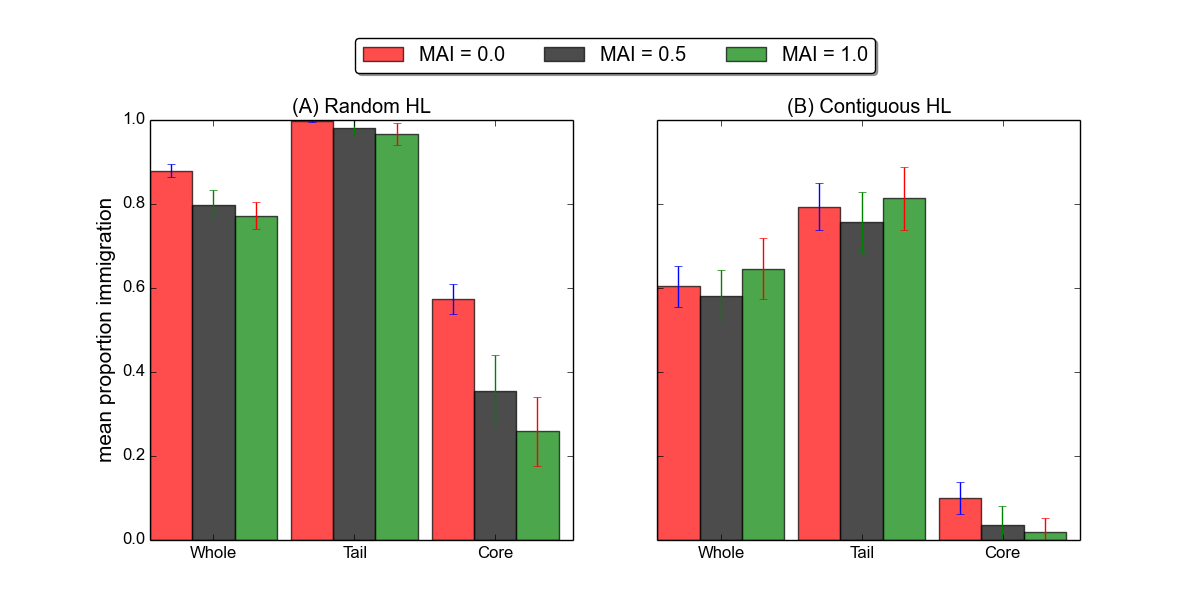
\includegraphics[width=\textwidth]{{{figures/bivariate_v_HL/dependence_IR_core_tail}}}
%	\caption{\textbf{Dependence on immigration} at HL$=90\%$, split into tail, core and whole community.}
%	\label{fig:biv_HL_tail_core}
%\end{figure}
%
%
%
%From figure \ref{fig:biv_HL_proportion_im} we see that the dependence on immigration is lower across the HL gradient than was observed when using the default IR. This can 
%
%Figure \ref{fig:biv_HL_proportion_im} shows the mean dependence on immigration:
%\begin{itemize}
%	\item In both cases dependence on immigration is lower than in chapter \ref{chap:}, which makes sense since the IR is lower.
%	\item In the random scenario HL increases dependence on immigration for all MAI ratios. As in first chapter.
%	\item This explains the increase in evenness within trophic levels, and the community level response of the antagonistic communities. However it does not explain the community level decrease in evenness of antagonistic communities  - this must be due to differences between trophic levels (or functional groups). For example plants become much more abundant relative to other groups. (See relative abundance plots below). 
%	\item In the contiguous scenario there is a very slight increase in dependence on immigration. 
%	\item Therefore we cannot explain the decrease in evenness under contiguous HL, which is especially pronounced for antagonistic communities. It is also clear the dependence on immigration \emph{is not to only determinant of evenness}.\footnote{The converse is that dependence in interactions reduces evenness? Also we know that mutualism reduces evenness..but these communities don't get less even. They are less even to start off with.}  
%\end{itemize}
%
%\begin{figure}
%	\centering	
%	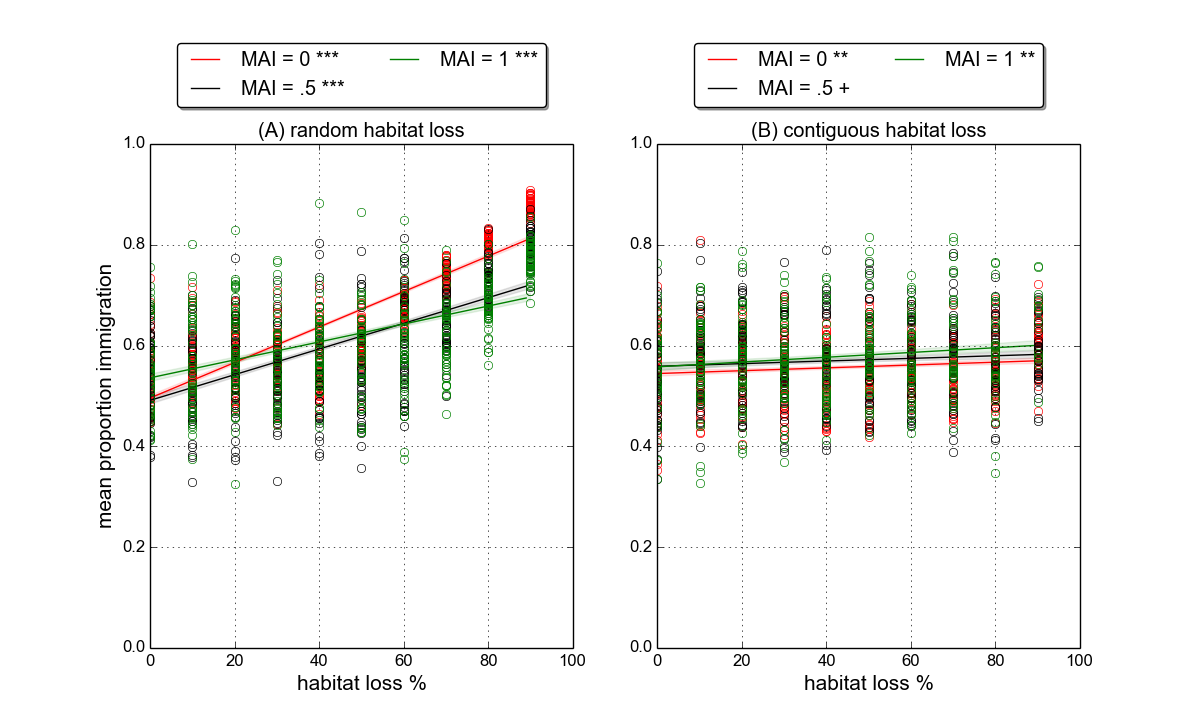
\includegraphics[width=\textwidth]{{{figures/bivariate_v_HL/lm_mean_proportion_immigration_3mai}}}
%	\caption{\textbf{Number of immigrants} as a fraction of the total number of new individuals created over the course of a simulation. Linear fits and p-value markers as in previous plots (see caption of figure \ref{fig:WHEREFIRST}).}
%	\label{fig:biv_HL_proportion_im}
%\end{figure}
%Why do mutualistic communities display more extinctions? - less even..
%Why do mutualistic communities display fewer changes in evenness?

\section{Bivariate analysis: fixed HL}
\label{sec:biv_fixHL}

In this section we study communities along a gradient of IR, at fixed HL. An intermediate HL value of $40\%$ was selected such that \emph{some} of the effects of habitat loss are present in the communities studied (see section \ref{sec:questions}). For an intuition of the state of the landscape at $40\%$ HL see figure \ref{fig:diffusion_example} (and the relevant animations at \cite{mcwilliams2015anim}). The analysis in this section addresses the following two observations from earlier in the chapter:
% This allows us to draw comparisons between the two HL scenarios, without being at the extreme of either scenario. 
\begin{enumerate}
	\item The total number of individuals in mutualistic communities appears to be insensitive to IR (figures \ref{fig:vir_diversity_random_hp} and \ref{fig:vir_diversity_contiguous_hp}).
	\item The total number of individuals in antagonistic communities increases at the lowest IR values (section \ref{sec:vir_diversity}), but this is not matched by a corresponding increase in the total number of interactions (section \ref{sec:vir_variability}).
\end{enumerate}

%There are certain features of the summary results from section \ref{sec:init_res} that make it desirable to study communities along an IR gradient at fixed HL. In particular the observation that mutualistic communities do not change total abundance with IR is interesting. We are also interested in why interaction strengths change in response to IR, and why total abundance increases at low IR for antagonistic communities.
%
%We may also be interested in the fact that reducing the IR does not necessarily reduce the dependence in immigration in a linear way - this is more subtle than we had previously imagined. It does reduce dependence until very low IR, when dependence suddenly increases again -perhaps due to the fact that there are too few individuals in the landscape to interact? Or perhaps because at these very low IRs a few species dominate, the majority of species just depend on immigrations.
%
%Plots to produce:
%\begin{itemize}
%	\item Relative abundance by FG
%	\item Possibly: RADs -> show that plants dominate, causing increase in abundance
%	\item Interaction strength distributions for shifting IR - probably conclude that this is the same feature is variability - metrics tends to infinity at low abundance
%\end{itemize}

\begin{figure}
	\centering	
	\includegraphics[width=\textwidth]{{{figures/bivariate_v_IR/example_RADS_mai0_random}}}
	\caption{Similar to figure \ref{fig:biv_HL_rads_mai0_random}, but for three different IR values. In all cases \textbf{HL}$\mathbf{=40\%}$. These RADs are for \textbf{antagonistic communities} (MAI$=0.0$), under \textbf{random HL}.}
	\label{fig:biv_IR_rads_mai0_random}
\end{figure}
\begin{figure}
	\centering	
	\includegraphics[width=\textwidth]{{{figures/bivariate_v_IR/example_RADS_mai0_contiguous}}}
	\caption{Similar to figure \ref{fig:biv_HL_rads_mai0_random}, but for three different IR values. In all cases \textbf{HL}$\mathbf{=40\%}$. These RADs are for \textbf{antagonistic communities} (MAI$=0.0$), under \textbf{contiguous HL}.}
	\label{fig:biv_IR_rads_mai0_contiguous}
\end{figure}

\begin{figure}
	\centering	
	\includegraphics[width=\textwidth]{{{figures/bivariate_v_IR/example_RADS_mai1_random}}}
	\caption{Similar to figure \ref{fig:biv_HL_rads_mai0_random}, but for three different IR values. In all cases \textbf{HL}$\mathbf{=40\%}$. These RADs are for \textbf{mutualistic communities} (MAI$=1.0$), under \textbf{random HL}.}
	\label{fig:biv_IR_rads_mai1_random}
\end{figure}
\begin{figure}
	\centering	
	\includegraphics[width=\textwidth]{{{figures/bivariate_v_IR/example_RADS_mai1_contiguous}}}
	\caption{Similar to figure \ref{fig:biv_HL_rads_mai0_random}, but for three different IR values. In all cases \textbf{HL}$\mathbf{=40\%}$. These RADs are for \textbf{mutualistic communities} (MAI$=1.0$), under \textbf{contiguous HL}.}
	\label{fig:biv_IR_rads_mai1_contiguous}
\end{figure}

Both observations can be understood by looking at rank-abundance distributions (RADs) for communities at different IR values. RADs are plotted at three IR values: the lowest IR (0.0001), the highest IR (0.005), and the intermediate IR (0.0005) which was used in the previous section. Figures \ref{fig:biv_IR_rads_mai0_random} and \ref{fig:biv_IR_rads_mai0_contiguous} show RADs for antagonistic communities at $40\%$ random and contiguous HL respectively. At the lowest IR (panel A) the RADs are uneven and discontinuous, and the communities are dominated by plant species. This confirms our prediction from section \ref{sec:vir_variability} that the increase in abundance of antagonistic communities at very low IRs is due to an increased dominance of plants. At IR$=0.0001$ in both types of habitat (random and contiguous), non-basal species struggle to maintain viable populations that can interact with and make use of the high availability of plant biomass. This is consistent with results from section \ref{sec:closed_communities} where it was observed that communities without immigration are characterised by mass extinctions in non-basal levels, even in pristine landscapes. Increasing the IR makes the RADs more even. At IR$=0.0005$  (panel B) communities are still dominated by plant species, but the discontinuity between core and tail species is reduced. At IR$=0.005$ the communities are more even still and more non-basal species are present in the lowest ranks.  

Figures \ref{fig:biv_IR_rads_mai1_random} and \ref{fig:biv_IR_rads_mai1_contiguous} show RADs for mutualistic communities at $40\%$ random and contiguous HL respectively. At the lowest IR (panel A) the RADs are uneven and species persistent is low. In both types of landscape there are only around 30 species present in the community. In the random landscape the core of species consists only of plants and a single species from the second trophic level, which must be a mutualistic-animal. None of the benefit of mutualism is conferred to other species due to the nature of random HL, as we have seen previously (section \ref{sec:biv_HL_RADs}). In the contiguous landscape the core is more diverse, with species from all trophic levels, as we would expect due to the stronger species interactions in such a landscape. In both the random and contiguous cases we again see that increasing IR makes the RADs more even, which by now is a familiar result. Despite the very different characteristics of the RADs, the total number of individuals is approximately equal in all six communities displayed (as discussed in section \ref{sec:vir_diversity}). We see that the constant number of individuals in mutualistic communities is due to the dominance of a core of species, which may or may not contain species from all trophic levels depending on the type of HL. Increasing the immigration rate serves to increase diversity by reducing the dominance of the mutualistic core, and promoting evenness in the RADs, whilst maintaining the same total abundance.

%As stated we will investigate alternative definitions of extinction. These are the possible definitions:
%\begin{itemize}
%	\item Species that do no have any natural births (during a time period) i.e. only immigration, if any
%	\item Species that do not interact with other species during a time period
%	\item Species that are below a certain threshold (relative) abundance
%\end{itemize}
%
%We suspect that these different metrics will given similar results. Here we plot heatmaps based on the above three definitions.

\section{Discussion}
\label{sec:vir_discussion}

%Are species `in the tail' interacting at all?

The main goal of this chapter was to determine how community responses to the two habitat loss (HL) scenarios differed from those seen in chapter \ref{chap:habitat_loss_high_immigration} when the immigration rate parameter (IR) was reduced. In particular, given that the loss of habitat in nature leads to the loss of species, we were interested to find IR values at which HL produced species extinctions. Also, given the importance of the immigration mechanism in driving structural properties such as evenness (chapter \ref{chap:habitat_loss_high_immigration}), and dynamical properties such as variability and determinism (chapter \ref{chap:stress_testing}), we were motivated to study such properties systematically over a large region of parameter space. The analysis has generally furthered our understanding of communities simulated using the IBM model. We have found certain results to be consistent with those of chapter \ref{chap:habitat_loss_high_immigration}, and which therefore appear to represent robust features of the model. We have also presented certain new and unexpected results, which provide fresh insight into the workings of the model. The key results, falling into both of the aforementioned categories, are discussed in turn below before considering the ecological significance of these results in the conclusion (section \ref{sec:vir_conclusion}). 

Strong species interactions are associated with high temporal variability in population dynamics. This result was evident from the previous two chapters, and is robust across the region of parameter space explored here (section \ref{sec:vir_variability}). Random HL serves to reduce species interaction strengths, and therefore reduces temporal variability. The converse holds for contiguous HL. In general reducing the IR increase temporal variability (in agreement with chapter \ref{chap:stress_testing}), and slightly increases interaction strengths. Both the metric for temporal variability (mean CV) and for interaction strength (IS) tend to infinity in the limit that species abundance tends to zero. This property of the metrics must be considered in situations where species abundances are low, especially given the discrete nature of the model (species abundance must be integer valued). Specifically this limit behaviour appears to be an issue for \emph{IS} at the lowest IR value (both scenarios), and for \emph{mean CV} at high levels of random HL.

Immigration is a key feature of the model. The role of immigration in promoting evenness and reducing temporal variability were first observed in chapters \ref{chap:habitat_loss_high_immigration} and \ref{chap:stress_testing}. Both observations hold across this region of parameter space (sections \ref{sec:vir_diversity}, \ref{sec:vir_variability} and \ref{sec:biv_HL_evenness}). The fact that immigration prevents species extinctions has also been confirmed, since lowering IR was found to produce species extinctions (section \ref{sec:vir_diversity}). However extinction patterns were found to differ between the contiguous and random scenario. 

In general contiguous HL produces more extinctions than random HL (section \ref{sec:vir_diversity}). Also the number of extinctions due to contiguous HL is clearly dependent on the level of destruction, whereas under random HL this is only the case for antagonistic communities. At the reduced IR of $0.0005$ random HL does result in uneven communities with discontinuous RADs (section \ref{sec:biv_HL_RADs}). And under both types of habitat loss predator species (top two trophic levels) suffer due to increase levels destruction (section \ref{sec:biv_HL_RAFG}). However the low abundance species in the tail of the RAD are less vulnerable to extinction under random HL than contiguous. Under contiguous HL communities became less even (at the IR$=0.0005$) and many species in the tail go extinct. This results from the strong trophic interactions, characteristic of the contiguous scenario, which drive species to extinction. In contrast random HL produces weak interactions, and as such rare species are subject to less predation pressure from the more abundant species. 

In this chapter we have seen marked difference between mutualistic and antagonistic communities. As discussed previously mutualistic communities are less even (chapter \ref{chap:habitat_loss_high_immigration} and \cite{lurgi2015effects}). One consequence of this is that mutualistic communities exhibit more extinctions that antagonistic ones (section \ref{sec:vir_diversity}). Under random HL at low IR these extinctions are seen even in pristine landscape, where trophic interactions remain strong, and may be reduced by the onset of HL which reduces interaction strengths. Under contiguous HL mutualistic communities only exhibit more extinctions from increased HL, since trophic interaction strengths are increased. Extending the findings of chapter \ref{chap:stress_testing}, it is now clear that the lower evenness of mutualistic communities results from the dominance of a core group of species (section \ref{sec:biv_HL_RADs}, \ref{sec:biv_fixHL}). Depending on the context this core group may contain non-mutualistic species which benefit as a by-product of mutualism. The core group is also able to maintain the total abundance of the community as a whole in the face of changing IR (section \ref{sec:vir_diversity}), by increasing its dominance (section \ref{sec:biv_fixHL}). Increased IR serves to reduce the dominance of the core group and allow competing species to prosper.

In section \ref{sec:biv_netprops} we saw that network properties (quantitative generality and vulnerability) may change under both types of HL at low immigration rates (IR$=0.0005$). This represents a departure from the results of chapter \ref{chap:habitat_loss_high_immigration}, where only random HL produced significant changes in network properties. In general the observed changes in network properties are consistent with the conclusion that they are largely driven by changes in the distribution of species abundances (characterised by \emph{evenness}). However the species extinctions, observed at reduced IR, may also contribute to changes in network properties. Further analysis would be required in order to fully understand the mechanisms that drive changes in the structure of the realised interaction network. We do not pursue such an analysis in this thesis. We conclude that network properties may indeed change in response to HL, in ways that are related to other changes in the community. Therefore such properties represent useful indicators of the impact of HL. However sole focus on network properties may obscure some of the effects of HL. For example, network properties did not change under contiguous HL at high IR (chapter \ref{chap:habitat_loss_high_immigration}), despite significant changes in interaction strengths (IS) and a loss of temporal stability.    

%In contrast 
%
%Random HL appears to be beneficial to low abundance species, in that they are not driven to extinction by predation/competition. However this benefit is only realised in the presence of immigration. As we saw in chapter \ref{chap:}, without immigration these species would be driven to extinction.
%
%..In chapter \ref{chap:hhl} we saw that species abundances became more even under random HL, while they evenness did not change significantly under contiguous HL. These changes we attributed to the dependence of communities on immigration, which acts to make the distribution of individuals across species more even. Therefore we expected that at low IR we may observe a change in the evenness response. The IR of $0.0005$ was chosen because it appeared to generate communities that became less even under contiguous HL, especially in the case of MAI$=0.0$.
%
%Given what we know about random HL to dominance of plants at high HL is easily explained by lack of grazing!
%
%We conclude that mutualism benefits some species, and not just those that interact mutualistically, but also those that feed on them. However this benefit is restricted to a few species, while others suffer from the increased fitness of their competitors. Immigration acts to reduce the disprecpacny between the two groups. And random HL reduces the benefit of mutualism to species in higher trophic levels, because less energy is passed up the food chains. 
%
%In mutualistic community random HL can reduce extinctions by..
%
%The drivers of changes in network properties are numerous, and mechanism behind the same changes may differn between HL scenraio and MAi ratios, making interpretation difficult.

\section{Conclusion and perspectives}
\label{sec:vir_conclusion}
\footnote{Some of this material might be better in final conclusion chapter. Although here seems appropriate before moving on to a slightly different topic.}

From the analysis in this chapter, and chapter \ref{chap:habitat_loss_high_immigration}, it is clear that mutualism plays an important role in shaping communities and mediating their response to HL. In general we have observed that mutualism reduces the evennness of communities, and it appears that this is due to a dominant core of species which benefit either directly or indirectly from mutualism (sections \ref{sec:biv_fixIR} and \ref{sec:biv_fixHL}). Two recent empirical studies have detected a similar effect in natural systems. The presence of a \emph{resource mutualism} between plants and root fungi was experimentally manipulated in a field study by Rudgers et al. \cite{rudgers2008invasive}, and in a mesocosm experiment by Keller \cite{keller2014mutualistic}. Both studies determined that the presence of mutualism had negative effects on the diversity of the plant community as a whole, resulting from increased dominance of the plant mutualists. In \cite{keller2014mutualistic} the mutualism was found to increase total plant productivity on aggregate, despite the decrease in diversity. In \cite{rudgers2008invasive} the effect of mutualism was seen to propagate to higher trophic levels, reducing the diversity of arthropod species. Our results are in agreement with these observations. Furthermore	they suggest that the diversity-reducing effect of mutualism changes community response to habitat loss, leading to a larger number of extinctions due to the reduced fitness of non-mutualistic competitors. 

Our findings support previous theoretical results that the effects of HL are mediated by the spatial pattern in which habitat is destroyed \cite{allen2007self,jager2006simulated,dytham1995effect,
hill1999habitat,travis2003climate,with1999extinction,ovaskainen2002metapopulation}. The most general result from the studies cited is that habitat lost in some spatially-correlated manner is less detrimental than habitat lost at random (in terms of the number of expected extinctions). The reasoning for this is that spatially-correlated loss leaves larger areas of pristine habitat in tact. We have compared two patterns of HL: random and contiguous. Our treatment represent a detailed investigation of the matter because the modelling spatially-explicit, individual based, and multi-trophic. The results do not entirely agree with previous modelling. In particular contiguous HL was found to produce more extinctions than random HL, and was also more damaging in terms of dynamic stability. In contrast random HL showed the potential to produce \emph{trophic collapse}, because destroyed landscape cells provided barriers to motion reducing the ability of individuals to find interaction partners. In some cases random HL produced communities that were almost entirely dependent on immigration to persist.

The observed responses of communities under contiguous HL are consistent with those derived from a meta-community model by McCann et al. \cite{mccann2005dynamics}. Their model showed that \emph{spatial compression} of communities may result in strong predation by organisms in higher trophic levels, with a destabilising effect in the local communities. Perhaps the most significant difference between our model and theirs is the mechanism by which predator species are able to persist in highly impacted landscapes. In our model this mechanism is immigration (see chapter \ref{chap:stress_testing}, in theirs it is mobility of the predator between different patches. However the destabilising effect of predation is the same. There is some empirical evidence that increased temporal variability is present at the edge of forest fragments \cite{ewers2006continuous}. Gonzalez et al. \cite{gonzalez2011disentangled} suggest that this effect may be due to increased interaction strengths, although they stress the need for empirical studies to confirm this hypothesis. Our findings support the call for empirical studies in this area.\footnote{Can also talk about variability-area relationship here, if not already discussed?}.

In general our model suggests that strong trophic interactions are destabilising. This conclusion is supported by a wealth of previous theoretical studies (from \cite{may1972will} to \cite{mccann1998weak} and \cite{neutel2002stability}), and by the empirical work of O`Gorman \cite{o2009perturbations}. We have seen that strong interactions produce variable population dynamics, reduce the evenness of the community, and drive species extinctions in the case of contiguous HL. There is also evidence (chapter \ref{chap:stress_testing}) that trophic interactions drive resource competition in simulated communities. However we have not modelled competitive interactions directly. Coyte et al. have recently suggested that such interactions may be key in stabilising communities \cite{coyte2015ecology}, and their inclusion in the IBM may present in interesting avenue for further study. In general we have not found evidence that the introduction of mutualism stabilises the dynamics of communities with strong atagonistic interactions, as suggested by Mougi et al. \cite{mougi2012diversity}. In fact, as discussed above, mutualism has proven to be harmful to communities in many ways.

Throughout chapters \ref{chap:habitat_loss_high_immigration} to \ref{chap:varying_immigration_rate} immigration has been revealed as a key factor in the IBM. The immigration mechanism, as we model it, drives evenness in species abundances and their distribution across space. Immigration may also counter the effects of mutualism (by reducing the dominance of the mutualistic core), and dampen the temporal variability associated with strong species interactions. It may also mitigate some of the effects of HL, in particular by preventing the extinction of species. However, in this chapter, we have shown that there is a subtle interplay between immigration and the response of community properties (such as evenness) to HL. In many ways the response of communities at low levels of immigration (IR$=0.0005$) was more \emph{realistic} than those observed at the \emph{default IR}. Specifically HL resulted in species extinctions; predator populations suffered under both types of HL; and evenness decreased in some cases (representing a loss of diversity). These findings suggest that the \emph{default IR value} may be artificially high compared that of natural communities. 

It is clear, from chapter \ref{chap:stress_testing}, that some non-zero IR is required for the IBM to produce persistent and diverse communities. Such a situation may not be \emph{unrealistic}. As discussed in section \ref{sec:intro_community_ecology}, the study of local communities in isolation from their surroundings is an abstraction of nature. In \cite{ricklefs2008disintegration} Rickelfs argues that not only must we consider larger areas of space in order to understand biodiversity at a regional scale, but we must consider influence from different localities in order to understand any single local assemblage of species. Hence the popularity of the meta-community concept \cite{leibold2004metacommunity}, and the associated class of models (for example \cite{ovaskainen2002metapopulation}). The immigration mechanism of the IBM models such connectance of the local community with other parts of the landscape. Given the importance of immigration, and the simplicity of the mechanism by which we model it, this seems a natural candidate for further development of the IBM. One possibility would be to introduce differential rates of IR for species in different trophic levels (this would account for the fact that larger species tend to be more mobile). An alternative, and more computationally expensive option, would be to simulate numerous communities in parallel and allow dispersal of individuals between different landscapes. In either case, changes to the way that immigration is modelled would likely affect simulated community responses to HL. 

In this chapter and chapter \ref{chap:habitat_loss_high_immigration} we have seen that network properties may change in response to HL. We have argued that, in the IBM simulations, the changes in network properties are largely driven by changes in the distribution of species abundances. Therefore in this chapter we have focused more closely on properties relating to species abundances and on stability. However the ability to study network properties and how they relate to other aspects of simulated communities is a powerful feature of the IBM. Therefore further investigation on this topic represents more scope for future development. It would be informative to use statistical methods to quantify the mechanisms that drive changes in network structure\footnote{SEM models?}. It would also be possible to ask explicit questions about the role of network structure in generating community properties (such as stability). This possibility was touched on in chapter \ref{chap:stress_testing}. By using interaction networks with pre-defined properties (for example modularity or nestedness), or even empirically derived networks, it would be possible to gain more insight into the role different structural properties. 

%\begin{itemize}
%	\item Importance of immigration may hold true (ref. meta-community theory)
%	\item Similarly the role of species interactions as a destabilising force (reduce evenness, create competition, increase variability), may also hold true. Ref: competitive exclusion. Although mention other other resolutions: endogenous factors due to interactions suggested weak compared to exogenous factors (e.g. environmental variability). Differential species traits. Phylogeny.
%
%	\item Regarding extinctions our findings disagree with many theoretical studies - we get more extinctions due to contiguous than random HL. 
%
%	\item Network metrics did not prove particularly informative in understanding community responses, disagreeing with many other studies. 
%	\item On the whole the response of communities at low IR (0.0005) seems more realistic than at high IR (0.005) - species go extinct, evenness can decrease, predator suffer in both random and contiguous scenario.
%	\item However there are certain limitations in the model that may see a departure from our results in future empirical studies - these are discussed in (conclusion chapter?) 
%\end{itemize}

%\newpage
%\section{Exploration of parameter space: habitat loss and immigration}
%\label{sec:heatmaps}
%
%\begin{figure}
%	%\centering	
%	\hspace{-2.5cm}
%	\includegraphics[width=1.3\linewidth]{"./chapters/chapter04/figures/init_proportions"}
%	\caption{Mean number of species belonging to each functional group for the three MAI ratios in consideration ($0.0,0.5,1.0$). The results are averaged over one thousand simulations with the given MAI ratio, selected from the total ensemble of simulations that were run for this chapter (and used to generate e.g. fig \ref{fig:summary_heatmaps_imvshl}). The species numbers depicted are independent of all simulation parameters, other than those that define the interaction network. That is the average number of species in each function group depends on the niche model parameters (connection and number of species ), the MAI ratio, and the trophic constraints that we impose. }
%	\label{fig:initial_proportions}
%\end{figure}
%
%
%% In order to do what exactly...?
%Motivated by the above we explore a two dimensional slice of parameter space. The immigration rate (IR) and the level of habitat destruction (HL) are varied and one hundred repeat simulations are conducted at each pair value. Therefore were are able to estimate how the simulated communities are expected to behave across this region of parameter space, by averaging over the repeats. These simulation are run for three different MAI ratios: 0.0, 0.5 and 1.0. As in previous simulations each repeat uses a different interaction network topology, generated with the procedure described in section \ref{sec:whereis}.  All other parameters are held constant at their default values (table \ref{tab:wehereis}), including the number of iterations which remains at 5000. 
%
%In order to speed up the simulations certain metrics used in the previous analysis (chapter \ref{ch:whereis}) are not calculated. Particulary the spatial stability metrics are computationally expensive. Only two pieces of information are saved as output from these simulations: the underlying network structure and the abundance time-series for each species. The abundance time-series is simply a record of the abundance of each species at every simulation iteration. (What do we calculate from these and why..) By limiting the simulation output the scope for analysis is restricted but the parameter space can be explored in more detail (higher resolution, greater number of repeats)\footnote{The changes to the model output reduced run times by up to a factor of 10. This required changes in how the interaction network is represented and therefore previously used network metrics could not be calculated. However it would be easy to modify the code to save some information on interaction frequencies and spatial states, which could be used in later analysis. This has not been done yet -ON THE WAY.}. This `first pass' scan of the parameter space allows us to construct a general picture of how the model behaves in this region. It may also be used to identify subsets of the  region of parameter space on which to focus further computational effort for e.g. spatial analysis.
%
%The entire range of habitat destruction is explored from pristine landscape ($0\% HL$) to near total destruction ($90\%HL$) in steps of $10\%$. In the current chapter all habitat is destroyed using the contiguous algorithm since it was decided that this is more realistic (see discussion in section \ref{sec:whereis}). Ranges for the IR were chosen based on previous simulations. Since $IR=0.005$ is sufficiently high to prevent any extinctions, this was taken as the maximum of the range. Simulations using $IR=0$ have already determined that this leads to community collapse, therefore these were not repeated. A value of $IR=0.0001$ was heuristically selected as the lower bound, at which some non-zero extinction is expected in pristine habitat for all MAI ratios\footnote{Dani thinks we should maybe look at lower IR values.}.
%
%The choice of MAI ratios allows us to compare purely antagonistic ($MAI=0.0$), mixed ($MAI=0.5$) and purely mutualistic ($MAI=1.0$) communities. Figure \ref{fig:initial_proportions} shows the expected fraction of species belonging to each of the six functional groups in the interaction networks for these communities. The constraints we place upon the niche model are that at least $25\%$, $25\%$ and $5\%$ belong to the first, second and fourth trophic levels respectively. In particular it is known that the unconstrained niche model struggles to generate realistic number of species in the second trophic level [REF]. The figure shows that the interaction networks meet these constraints and that, as expected, the largest number of species is found in the third trophic level\footnote{Perhaps these constraints should be changed in future simulations - discuss with Daniel. - he thinks OK. Suggests look at RADS with colouring by TL. REQUIRES LOOKING AT SINGLE NETWORK.} i.e. the functional group labelled \emph{omnivores}. Antagonistic communities are missing the two mutualist functional groups from the first two trophic levels, whereas the mixed communities have a roughly $50:50$ split between mutualists and non-mutualists as expected (this split is not exact because it is links that are switched no species). Importantly although the purely mutualistic communities contain no herbivores (as all their links to plants have been switched), they do contain non-mutualist plants. These plants are those that share no interactions with the first trophic level\footnote{Is this realistic - Daniel? - RESTSAE QUESTION: REAlISTIC THAT PLANTS ARE NOT EATEN BY FIRST TROPHIC LEVEL..}, therefore the link replacement procedure does not give them any mutualist partners. These plants remain wind dispersed and are predated upon by animals from trophic levels three and four\footnote{Should there be a constraint that top predators do not consume plants? Not in original niche model. (Dani says no. Re-run. Does it make a difference?}.   
%
%%%%%%%%%%%%%%%%%%%%%%%%%%%%%%%%%%%%%%%%%%%%%%%%%%%%%%%%%%%%%%%%%%%%%%%%%%%%%%%%%%%%%%%%%%%%%%%%%%%%%%%
%%% Archetypal rotated figure page:
%%% STILL BEING A PAIN IN THE ARSE - NEEDS WORKING ON!
%%\newpage
%\clearpage
%%\afterpage{%
%\thispagestyle{empty}
%\begin{sidewaysfigure}
%
%		\centering      
%		\hspace{-3cm}
%
%        \includegraphics[width=\linewidth]{"./chapters/chapter04/figures/sum_maps"}
%        \caption{\textbf{Summary heat maps:} Each heat map shows the value of a certain response metric across a 2-dimensional slice of parameter space. The parameters varied are immigration rate $IR$ (y-axis) and percentage habitat destruction $HL$ (x-axis). Each row of plots corresponds to a different MAI ratio as labelled. To construct the heatmaps one hundred repeat simulations were run for each combination of parameter values, with each simulation using a different underlying network. The mean value of the response metrics is taken over the hundred repeats. Therefore each pixel shows an estimate of the expectation value of the metric at those parameter values. The left column shows the expected number of species that are extinct at the end of a simulation; the central column shows the expected biomass (total number of individuals) at the end of a simulation; and the right column shows the expected temporal variablity (coefficient of variaiton of total biomass) of the dynamics during the final thousand iterations of a simulation. The latter is used as a proxy for stability (see text).}\label{fig:summary_heatmaps_imvshl}
%        %% Note: this figure generated by Documents/IM_vs_HL_heatmap/plot_sum_maps.py
%\end{sidewaysfigure}
%\clearpage
%%}
%%%%%%%%%%%%%%%%%%%%%%%%%%%%%%%%%%%%%%%%%%%%%%%%%%%%%%%%%%%%%%%%%%%%%%%%%%%%%%%%%%%%%%%%%%%%%%%%%%%%%%%
%
%\subsection{Summary heat-maps}
%\label{sec:sum_heat_maps}
%
%The results of these simulations can be concisely represented as heat maps over the region of parameter space explored. Figure \ref{fig:summary_heatmaps_imvshl} shows how the expected value of three summary metrics varies across this space: the number of extinct species, community biomass (total number of individuals) and temporal variability in community biomass. The response of each of these metrics is discussed individually below. The latter is used as a proxy for stability and is measured by the coefficient of variation (CoV) of the community biomass about its mean during the final thousand iterations of a simulation. (later..) This metric is often used to assess dynamic stability, but should not be confused with rigorous mathematical metrics relating to the stability of the equilibrium state of the system [REF]. It should be noted that the other two metrics, and all abundance measures in the following analysis, are calculated from a snapshot of the system state on the final iteration of a simulation. (Dani points out that average over replicates.., compare with averaged analysis, and discuss in context of steady state.) 
%
%\subsubsection*{Extinctions}
%
%No species extinctions are expected for sufficiently high levels of IR, across the whole range of HL values and for all MAI ratios. This results is visible in the left column of figure \ref{fig:summary_heatmaps_imvshl} and was already discussed in section \ref{sec:whereis}. It is found that reducing the IR leads to an increasing number of extinctions. At low IR extinctions are possible, even in pristine landscape. This fits the previous observation that zero IR always leads to community collapse.
%
%Increasing HL generally increases the number of expected extinctions. However nowhere in the parameter space do we see community collapse. In the most extreme case of low IR and high HL ($MAI=1.0,HL=90,IR=0.0001$) an average of close to thirty extinctions may be expected. Although this expected loss of half of the species is fairly catastrophic, it does not guarantee total collapse of the community. The trophic constraints imposed in the food-web generation procedure ensure that at least $25\%$ of species belong in the first (basal) trophic level (figure \ref{fig:initial_proportions}). In practice this very rarely (quantify) reaches above $30\%$. Therefore a loss of thirty species suggests that at least $40\%$ of the remaining species are non-basal\footnote{If all thirty species lost are non-basal we are left with $3/5$ basal species to $2/5$ non-basal. IN NATURE HIGHER TROPHIC LEVELS USUALLY MORE VULNERABLE [REF]. IS THIS THE CASE. OOO, COMMUNITY COLLAPSE.}. In other words, despite significant loss of species, there is some persistence in higher trophic levels. 
%
%For all three MAI ratios there exists an IR where the expected number of extinctions is zero in pristine landscape, but increases with HL. So although the immigration rescue effect prevents total community collapse, we do have a situation where HL can initiate species extinctions. The IR at which extinctions are initiated is increased by increasing the MAI ratio. This effect of MAI ratio on extinctions is general. On average we expect a greater number of extinctions for high MAI (1.0) than for low MAI ratio (0.0), all else being equal. At the lowest IR and with pristine habitat we may expect about one extinction with a MAI ratio of 0.0, compared to about ten extinctions with a MAI ratio of 1.0. This can possibly be explained by looking at the second column in figure \ref{fig:summary_heatmaps_imvshl}. On average a higher MAI ratio lead to a greater total number of individuals at the end of a simulation\footnote{Mechanism behind this? - From the Theoretical Ecology paper: "communities with larger MAI ratios hosted a larger number of individuals $(F(1273) = 98.69, p < 0.001)$ (Fig. 4). In spite of a decline in the abundance of non-mutualistic primary producers and herbivores with increasing MAI ratios (as expected due to a larger fraction of mutualistic species), the increase in mutualistic plants and animals overcompensated for this loss, causing an overall increase in abundance. This overcompensation was due to mutualistic plants becoming more abundant than non-mutualistic ones since mutualistic consumers do not consume as much resources from them and are, additionally, beneficial for their reproduction.}. This means that there are fewer empty landscape cells into which an individual may immigrate at random. This reduces the \emph{effective immigration rate} and so weakens the rescue effect. Any very rare species, only made viable by immigration, will be the ones hit by this and are likely to go extinct\footnote{To determine if this is what is happening need to look at total abundances?}. 
%
%\subsubsection*{Community biomass}
%%\label{sec:com_bio}
%There are strong trends in expected community biomass. Increasing HL has a negative effect on community biomass. This is intuitive and has been seen before. Also previously discussed (chapter \ref{ch:whereis}) is the result that, on average, communities with higher MAI ratio can support a greater biomass. However this effect is striking in these results, especially at low levels of HL. In a pristine habitat with an IR of 0.005, the expected number of individuals for a community with $MAI=0.0$ is around $20,000$, compared to around $50,000$ for a community with $MAI=1.0$. In fact, across the parameter space, purely mutualistic communities have around twice the biomass of purely antagonistic ones. Therefore in some sense mutualism appears to be `better' for the community. (Dani: although having more individuals means rescue effect less likely, and perhaps increase competition for space)  In section \ref{sec:whereis} we discuss whether it is better for the community as a whole, or only for those species that engage in mutualistic interactions.
%
%For antagonistic communities ($MAI=0.0$) the biomass is dependent on IR. Both very high and very low IRs support high biomass, whereas intermediate IRs support less (central panel, top row, figure \ref{fig:summary_heatmaps_imvshl}). The effect of high IR is intuitive - births due to high immigration supplement births due to reproduction in the local community. This supplementary effect is greater at higer IR. However the increase in biomass at very low IR is harder to explain. We know that at zero IR all non-plant species go extinct [REF CHPAT/SEC]. So we may expect that in the region of low IR non-plant species become increasingly rare\footnote{This can be checked later..}. In an antagonistic community this means a reduction in the number of herbivores and omnivores, which will benefit plant species. Therefore we may propose that the increase in the biomass at low IR is accounted for by an increased abundance of plants\footnote{This proposed mechanism may be working in reverse in the MAI=1.0 communities.}. This reasoning suggests that we should expect a difference in composition between the abundant antagonistic communities seen at low and high IR (see section \ref{whereis} - ABUNDANCE DISTS.).    
%
%Mutualism removes the dependence of community biomass on IR. Although the total biomass does not vary with IR for these communities ($MAI=0.5,1.0$) there may be changes in community composition. For example it is still reasonable to suspect that non-plant species become increasingly rare at low IR. However in a mutualistic community this has a different effect. It will benefit those plants that still have antagonistic interactions, but it will be detrimental to mutualist plants since they will be less likely to interact with a partner and therefore less likely to reproduce. So we may expect a shift in the relative abundances of the two functional groups of plants in favour of the antagonists at low IR (see section \ref{sec:rel_abun}).
%
%%% INCLUDE ELSEWHERE?? This is because the immigration mechanism provides a significant recovery effect.   It allows species that have gone locally extinct (from the simulation landscape) to recover by occupying empty cells. Therefore, for immigration values close to those used in the original simulations (chapter \ref{sec:where}), the average number of species that have gone extinct at the end of a simulation is close to zero\footnote{Since it is possible for a species to go extinct and to subsequently recover it may be sensible to use another definition of 'extinct'.}. This is true for all MAI ratios as shown by the left 
%
%\subsubsection*{Temporal variation}
%%\label{sec:temp_var}
% 
%In general increasing HL increases the temporal variablity of the dynamics. That is, communities are less stable in damaged landscapes. This result is only seen in the case of contiguous habitat destruction, as opposed to random destruction, and is discussed in more detail in section \ref{sec:wehreis} where it was shown to be associated with changes in the distribution of interaction strengths. Also communities are less stable at lower IR. This fits with previous results. It has been shown that communities are very stable and resistant to HL at high IR (section \ref{sec:whereis}). It has also been shown that they are unstable at zero IR, exhibiting community collapse (section \ref{sec:whereis}). This suggests that the model has a stable and an unstable regime, and that there must be a transition between the two when moving form high to low IR. The right-hand column of figure \ref{fig:summary_heatmaps_imvshl} shows a signature of this. Interestingly the loss of dynamic stability is greatest for antagonistic communities and weakest for purely mutualistic communities. This suggests that mutualism has a stabilising affect on community dynamics. It appears to confer better dynamic stability in the face of HL and changing IR (but there are also more extinction as discussed..).
%
%Another interesting feature of the CoV plots is that the trends described above appear to be broken at very low IR and high HL, where an increase in stability is visible. One potential mechanism is that this is an averaging effect. If some communities are totally collapsing in this region they would exhibit stable dominance of plant species, which would contribute positively to average community stability. However it may be that this effect is due to another mechanism.
%
%As mentioned previously the loss of dynamic stability is troubling since it calls into question the way that we calculate abundance metrics. Therefore the conclusions drawn in the following discussion may not be general and may not hold if the metrics were averaged over a number of iterations.(Dani: don't stress this here, put in limitations section.)
% 
% 
%\newpage
%\subsection{Example dynamics}
%\label{sec:example_dynamics}
%
%\begin{figure}[h!]
%	\centering	
%	%\hspace{-2.5cm}
%	\includegraphics[width=0.8\linewidth]{"./chapters/chapter04/figures/total_biomass_dynamics_hl_0_mai_0"}
%	\caption{Temporal dynamics of the total biomass of communities over the course of six simulations. Each panels shows the dynamics for three distinct simulations, each in a different colour. The left panels shows communities with a high immigration rate, and the right panel for a low immigration rate. In all cases there is no habitat destruction $HL=0$.}
%	\label{fig:total_biomass_dynamics}
%\end{figure}
%
%
%Figure \ref{fig:total_biomass_dynamics} illustrates the loss of stability in passing from a high to a low IR regime. This transition was proposed in section \ref{sec:temp_var}. The dynamics of three example antagonistic communities are depicted for each regime. These communities were selected at random from the one hundred repeat simulations at these parameter values. Antagonistic communities are shown because the increase in temporal variability is greater for these than for those with mutualism (see figure \ref{fig:summary_heatmaps_imvshl}). 
%
%In the high IR regime, shown in the left-hand panel of figure \ref{fig:total_biomass_dynamics}, we see that the total biomass of each community undergoes an initial transience followed by a period of relative stability. It appears that, during this second period, the system is undergoing stochastic fluctuations about its stable equilibrium\footnote{Test for this?}. In the low IR regime, shown in the right-hand panel, we see that the community biomass exhibits large scale fluctuations throughout the course of the simulations. It is not clear from inspection that the system is being perturbed about a stable equilibrium.\footnote{I would rephrase this. For example: there are different explanations for this patter: (i) Explanation 1, (ii) Explanation 2.} It may be that the reduction in IR increases the length of the initial transience, and that the communities illustrated are yet to reach steady-state after 5000 iterations. Or it may be that these communities reach their steady-state, but that the stochastic fluctuations are amplified because the equilibria are less stable\footnote{Further mathematical analysis to try and determine this? - Final chapter on model fitting?}. 
%
%\begin{figure}
%	\centering	
%	%\renewcommand{\thesubfigure}{}
%	%\setlength{\subfloatlabelskip}{0pt}
%	%\hspace{-2.5cm}
%	\subbottom[]{\includegraphics[width=0.8\linewidth]{"./chapters/chapter04/figures/trophic_dynamics_example_hl0_mai0"}}
%	%\caption{The mean initial number of species belogning to each functional gropup.}
%	%\label{fig:trophic_dynamics_example}
%	\subbottom[]{\includegraphics[width=0.8\linewidth]{"./chapters/chapter04/figures/trophic_dynamics_example2_hl0_mai0"}}
%	\caption{Dynamics from four individual simulation runs, with biomasses aggregated by trophic level. Each panel represents the dynamics of a single simulation run. In all cases the MAI ratio is $0.0$, and there is \textbf{no habitat destruction} ($HL=0$).  The coloured lines represent the temporal dynamics of the biomass of each trophic level, as indicated in the legends. Two immigration scenarios are presented. \textbf{Left column: high immigration. Right column: low immigration.}}
%	\label{fig:trophic_dynamics_example}
%	
%\end{figure}
%
%Figure \ref{fig:trophic_dynamics_example} shows example dynamics by trophic level of four antagonistic communities in the high and low IR regimes. The left-hand panels depict two communities in the high IR regime. Again the initial transience is followed by a period of relative stability, which is consistent across trophic levels. It is clear from these two plots that the positions of the system's equilibria and the size of the fluctuations about it vary between simulations.  
%
%The right-hand panel of figure \ref{fig:trophic_dynamics_example} depicts two communities in the high IR regime. It is clear from inspection that the mean and the variance of the biomasses varies between trophic level, and between simulation. The lower plot shows dynamics dominated by species from the first trophic level, with large scale but decreasing amplitude fluctuations in the second trophic level. The upper plot shows perhaps even less stable dynamics with increasing amplitude fluctuations in the first and fourth trophic levels, and very low abundances in the intermediate trophic levels. In both simulations there are several instances where the biomass of an entire trophic level comes close to zero. However, as figure \ref{fig:summary_heatmaps_imvshl} shows, we should only expect around one extinct species at the end of a simulation at this IR. It must be that that immigration is preventing stochastic extinctions here\footnote{At this IR we would expect on average four immigrations per iteration, if the landscape were empty.}, by providing some buffering to populations at the low end of their biomass fluctuations and by rescuing those species that do go extinct\footnote{It would be interesting to look at the breakdown of these trophic dynamics by species - e.g. how synchronous are the different species in the same trophic level with each other.}.
%
%The breakdown of dynamics by trophic level demonstrates that the timing of measurement will affect the calculation of relative abundance metrics, and not just that of the aggregate community biomass. If the fluctuation in trophic biomass were more synchronous between levels, the timing of the measurement would be less significant. However the figure shows that even the ordering of trophic levels by abundance is dependent on time\footnote{This is beginning to look make the results seem invalid.}. Therefore further analysis should attempt to remove this time dependence by averaging biomasses over a number of iterations. The plots suggest that the increase in community biomass at low IR (discussed in section \ref{sec:com_bio}) may be a genuine effect. However it is hard to determine the contribution of the increased fluctuations without averaging the abundances over time.
%
%(There may be other points in parameter space where it would be informative to plot the dynamics...e.g. high mutualism region, temporally stable)
%(Could plot biomass dynamics, averaged over replicates?)
%
%\newpage
%\subsection{Relative abundances and abundance distributions}
%\label{sec:rel_abun}
%
%Contextualise - begin this section with the points made above that suggest useful to look at RADS.
%
%Figure \ref{fig:rel_abun_tl_mai_01} shows the mean relative abundance of each trophic level for antagonistic and mutualistic communities, across the parameter space.  For purely antagonistic communities the proportion of individuals in each trophic level varies strongly with IR and weakly with HL. At low IR antagonistic communities become dominated by plant species. This is in agreement with the mechanism proposed in section \ref{sec:com_bio}, whereby plants benefit from a scarcity of animal consumers at low IR. At high IR the distribution of biomass is much more even across trophic levels. In this region of parameter space the biomass of trophic levels one and four are roughly equal at around $30\%$, with the remaining $40\%$ of the biomass split fairly evenly between trophic levels two and three. This biomass distribution is not necessarily unrealistic for a community in nature, however it does not conform to the classic \emph{biomass pyramid} (see discussion in section \ref{sec:whereis}). In fact the distribution at low IR is much closer to the standard pyramid.
%
%Mutualistic communities (MAI=1.0) show much less variation in their trophic composition across the parameter space. The first two trophic levels are most abundant, with slightly more biomass in the first trophic level than the second. The third and the fourth trophic levels are much less abundant with around $20-30\%$ of the biomass split fairly evenly between them. This distribution is remarkably constant over the parameter space. Only at extreme levels of disturbance ($IR=0.0001, HL\geq 70 \%$) do the communities begin to be dominated by plants. 
%
%Figure \ref{fig:rel_abun_fg_mai_51} shows the mean relative abundance of each functional group for mutualistic communities with $MAI=0.5$ and $MAI=1.0$. As expected purely mutualistic communities are dominated by functional groups two and four (mutualistic producer and animals) across the whole region of parameter space. Functional groups five and six do relatively better at high IR and low HL. Whereas at low IR and high HL the relative abundance functional group 1 increases significantly. This is an indication of the shift in favour of antagonists, suggested in section \ref{sec:com_bio}, due to the low biomass making it hard for mutualists to reproduce and less likely that plants will be eaten. The same patterns are seen in the case of $MAI=0.5$, however the trends appear stronger since the relative abundances are less robust to changes in IR and HL.     
%
%
%
%\begin{figure}[h!]
%	\centering	
%	%\hspace{-2.5cm}
%	%\renewcommand{\thesubfigure}{}
%	%\setlength{\subfloatlabelskip}{0pt}
%	\subbottom[$MAI = 0.0$]{\includegraphics[width=0.8\linewidth]{"./chapters/chapter04/figures/rel_abun_tl_mai_0"}}
%	\subbottom[$MAI = 1.0$]{\includegraphics[width=0.8\linewidth]{"./chapters/chapter04/figures/rel_abun_tl_mai_1"}}
%	\caption{The relative abundance of species belonging to each of the four trophic levels. Above: MAI = 0.0. Below: MAI = 1.0. Each pixel on the heat maps corresponds to an average over one hundred repeat simulations at those parameter values. The abundances are measured at the end of each simualtion.}
%	\label{fig:rel_abun_tl_mai_01}
%\end{figure}
%
%
%\begin{figure}[h!]
%	\centering	
%	%\hspace{-2.5cm}
%	%\renewcommand{\thesubfigure}{}
%	%\setlength{\subfloatlabelskip}{0pt}
%	\subbottom[$MAI = 0.5$]{\includegraphics[width=0.9\linewidth]{"./chapters/chapter04/figures/rel_abun_fg_mai_5"}}
%	\subbottom[$MAI = 1.0$]{\includegraphics[width=0.9\linewidth]{"./chapters/chapter04/figures/rel_abun_fg_mai_1"}}
%	\caption{The relative abundance of species belonging to each of the six functional groups. Above: MAI = 0.5. Below: MAI = 1.0. Each pixel on the heat maps corresponds to an average over one hundred repeat simulations at those parameter values. The abundances are measured at the end of each simulation.}
%	\label{fig:rel_abun_fg_mai_51}
%\end{figure}
%
%\subsection{Rank abundance distributions}
%\label{sec:rads}
%
%These results, as with the other should be recalculated using averaged metrics.
%
%Figure \ref{fig:mean_rads} shows the mean rank abundance distributions for a range of IR and HL values. Communities with all three MAI ratios are shown in different colours. Across the parameter space mutualistic communities (blue) have less even distributions than antagonistic communities. This difference is more pronounced at low IR and high HL. 
%
%An interesting feature of the RADs is that some of them display an apparent discontinuity in the distribution. This is perhaps most pronounced in the bottom left panel of figure \ref{fig:mean_rads} ($IM=0.0001, HL=0, MAI=1.0$). A sigmoidal shape is a feature of log-normal abundance distributions and is often observed in natural communities [REF]. However this extreme case does not appear to fit. What is driving this distribution?  The `flat' section of low abundance species could be those species whose presence is sustained only by continuous immigration and which are therefore present in roughly equal abundances?   
%
%
%
%\clearpage
%\afterpage{%
%%\thispagestyle{empty}
%\begin{sidewaysfigure}
%
%		\centering      
%		\hspace{-3cm}
%
%        \includegraphics[width=0.9\linewidth]{"./chapters/chapter04/figures/single_rads"}
%        \caption{\textbf{Rank abundance distributions} for individual simulation runs, for nine different pair values of immigration rate and habitat destruction. Each dsitribution is for a single community at the end of an individual simulation run. The different colours correspond to different MAI ratios: red = 0.0; green = 0.5; blue = 1.0. And the different symbols correspond to different trophic levels: circle = 0; upwards triangle = 1; sqaure = 2; downwards traingle = 3.}
%        \label{fig:single_run_rads}
%        %% Note: this figure generated by Documents/IM_vs_HL_heatmap/plot_sum_maps.py
%\end{sidewaysfigure}
%}
%
%%\clearpage
%\afterpage{%
%\thispagestyle{empty}
%\begin{sidewaysfigure}
%
%		\centering      
%		\hspace{-3cm}
%
%        \includegraphics[width=0.9\linewidth]{"./chapters/chapter04/figures/mean_rads"}
%        \caption{\textbf{Average rank abundance distributions} over one hundred simulation runs, for nine different pair values of immigration rate and habitat destruction. Each dsitribution is calculated using the mean relative abundance of the ranked species, averaged over the final abundances of one hundred repeat simulations. The different colours correspond to different MAI ratios: red = 0.0; green = 0.5; blue = 1.0.}
%        \label{fig:mean_rads}
%        %% Note: this figure generated by Documents/IM_vs_HL_heatmap/plot_sum_maps.py
%\end{sidewaysfigure}
%}
%
%
%\section{Points for discussion (Rough Notes)}
%
%A comparison of the relative merits of being a mutualist versus a non-mutualist is worthwhile. Importantly it must be remembered that mutualistic interactions are also trophic interactions. In our case, energy is transferred from producer to animal. In nature for example the bee receives energy from the nectar, but also carries pollen to fertilise other flowers.  So there is some loss/detriment to the producer as well as the benefit of reproduction (These mechanisms are in place in the model through the bioenergetic parameters. Traditionally, simulating mutualistic communities has failed because the simulations ended in an 'orgy of mutual benefaction'). It is an interesting strategy from an evolutionary perspective...discuss this (with relation to link switching)?
%
%
%In the model species become mutualistic by having at least one of their links, in the antagonistic interaction network, switched for a mutualistic link. Table \ref{tab:parameters} shows the default parameter values used for most simulations. Lets consider the potential benefit of switching a single herbivorous link for a mutualistic link, for either party. If the plant is a non-mutualist it must impart 20\% of its energy to the offspring when reproducing (this happens with a probability of 0.01 on each iteration). It is also subject to lose 70\% when it is encountered by this herbivour. If it were to switch this herbviourous link for a mutualistic link it would only lose 25\% of its energy in the interaction, and it would pass on a seed that is almost guaranteed\footnote{Really? We could look at how many mutualistic interactions lead to a new individual. It would only not occur in very crowded situations.} to generate an offspring. Therefore the cost of reproducing is slightly increased for a mutualist, but the cost of interacting with an individual from the trophic level above is dramatically reduced. There is an additional benefit that the mutualistic reproduction can occur over a greater distance. The net gain loss of this change depends on the probability/rate of interactions. We should investigate this, however the results suggest that being a mutualist is of significant benefit to plants. (These mechanisms are in place in the model through the bioenergetic parameters. Traditionally, simulating mutualistic communities has failed because the simulations ended in an 'orgy of mutual benefaction')
%
%Question: in the above analysis are mutualistic plants are relatively more abundant than non-mutualistic ones, except in the case of high habitat loss or low immigration (when there are few enough mutualistic partners that interactions become infrequent?) 
%
%For animals there is no cost to carrying and spawning the seed of their mutualistic partners. The only change in the switching of mutalistic links is the amount of energy that they receive from the interaction. During a herbivourous interaction, the hebivore takes 70\% of the plant's energy, and assimilates it with an efficiency of 80\%. Therefore it obtains ~60\% of the plants energy. During a mutualistic interaction the animal-mutualist takes and assimilates 25\% of the plants energy. Therefore on an interaction by interaction basis there is a negative trade off for an animal in switching its link to mutualistic. However there may be an emergent benefit in that this type of interaction is much better for plants, therefore increasing the plant biomass and therefore indirectly benefiting animal (mutualists and non-mutualists?) due to the increased frequency of interactions (density of plants).       
%
%
%%% IMPORTANT POINTS:
%%\begin{itemize}
%%	\item Do mutualistic plants only reproduce mutualistically? (almost certain yes)
%%	\item Does MATINGRESOURCE apply to mutualistic interactions?
%%	\item Why are top predators able to eat plants?!! Does omnivory trade off apply?? - too many individuals belong to TL3 in general.
%%\end{itemize}
%
%
%Mutualism in general stabilises dynamics, and leads to communities with more realistic biomass pyramids - i.e. dominated by the first two trophic levels, with fewer individuals in TL2/3. 
%
%It could be argued that the RADS are realistic, and the some immigration is a requirement to prevent stochastic extinction of the very rare species, which are found in nature. This begs the question as to what mechanism prevents their extinction in nature? And are they the most vulnerable to extinction?  
%
%\section{Habitat loss with low immigration}
%
%\section{Questions for Alan or Daniel}
%
%\begin{itemize}
%	\item Worried about general flow and structure of discussion. Feels like trying to present too much information all at once. How to not turn into a list of facts, where the relevance gets lost?
%
%	\item Since the dynamics do not necessary reach steady state should I re-do analysis with average over a time window? (We need a discussion section where the results are discussed in the context of current literature in the field, real-world communities, etc. Also, contextualizing (see a previous comment) is important so the reader does not feel like we include all these metrics because we can. For doing this it is always helpful to write down the main findings as bullet points and develop them; also, the limitations of the model should be presented here as well as the ways forward)
%	\item Can I use "we"??
%	\item Tense?
%	\item Figure 1.1 summary heatmaps: too much information in one figure? (feels that way from discussion).
%	\item OK to use plant, basal and producer interchangeably?
%
%	\item The ability of the top predator to survive almost entirely on plant matter is troubling.
%	
%	\item Is it in fact OK to use biomass and number of individuals interchangeably? 	(We need a discussion section where the results are discussed in the context of current literature in the field, real-world communities, etc. Also, contextualizing (see a previous comment) is important so the reader does not feel like we include all these metrics because we can. For doing this it is always helpful to write down the main findings as bullet points and develop them; also, the limitations of the model should be presented here as well as the ways forward)
%	
%	%\item TODo: linear interactions? (should it be that freq/predabun should be linear in preyabun? Same gradient across species?) If so we should be able to fit a GLV, if not via Timme, then via repreated simulations and some numerical optimisation.
%	\item Theme for discussion seems to be developing: point out a feature of the results, explain what could be causing it (in the model), relate this to other results. (should add to this - comment on how this may relate to the real world??) (Agree. The discussion section to summarize and explain, contextualize the results is needed.)
%\end{itemize}
%
%RADS: Good. As the main changes are observed for different IR it is good to include plots of abundance vs rank with the lines representing different IRs. Also, it could be nice to see if they deviate from a classical lognormal or lognormal family type distribution (which is usually found in nature)
%
%Are the legends correct? The plots next to this note are similar. I think they have different IR, right?

